\documentclass[12pt,a4 paper]{extreport}
\usepackage{ryan}
\usepackage[bottom]{footmisc}
\usepackage{pdfpages}

\pagestyle{fancy}
\fancyhf{}
\fancyhead[L]{\leftmark}
\fancyhead[R]{\thepage}
\renewcommand{\headrulewidth}{0.4pt}
\renewcommand{\arraystretch}{1.2}

\begin{document}
\includepdf{cover_page_oly}
% https://docs.google.com/document/d/16kOeQzcc1JQYCoyodSDyo9ZaX-T8cB4_vS0aQazFpfc/edit?usp=sharing

\begin{titlepage}
\title{The Road to Mastery:\\
Mathematics Olympiad}
\author{Ryan Joo Rui An}
\date{Last updated: \today}
\end{titlepage}

\maketitle

\chapter*{Preface}
\section*{About the Author}
Ryan Joo Rui An is a high school student currently completing his A Levels in Singapore. He has participated in numerous Mathematics Olympiad competitions and consistently achieved decent results, including the Singapore Mathematics Olympiad (SMO) and IMO National Selection Test (IMONST), which are the two selection tests for the prestigious International Mathematics Olympiad (IMO) by Singapore and Malaysia respectively.

\section*{About the Book}
The motivation of the writer to write this book was to the author for Mathematics Olympiad competitions by summarising important topics in Mathematics Olympiad, with a focus on SMO and MAA-AMC, which feature rather challenging problems.

Do reach out to the author at \texttt{ryanjooruian18@gmail.com} if you wish to point out any (glaring) mistakes, or provide comments and suggestions regarding the content and/or formatting of the book.

\section*{Resources}
Here are some notes and materials that you might find useful when learning Mathematics Olympiad:
\begin{itemize}
\item \href{http://www.overleaf.comhttps://web.evanchen.cc/handouts/Syllabus/Syllabus.pdf}{Unofficial syllabus for math olympiads, by Evan Chen}
\item \href{https://web.evanchen.cc/handouts/english/english.pdf}{Notes on proof-writing style}
\item \href{https://artofproblemsolving.com/community/c13_contests}{AoPS Contest Collections}
\item \href{https://yufeizhao.com/olympiad/}{Yufei Zhao's olympiad handouts}
\item \href{https://web.evanchen.cc/olympiad.html}{Evan Chen's olympiad handouts}
\item \href{https://web.evanchen.cc/problems.html}{Olympiad Problems and Solutions, by Evan Chen}
\item \href{https://cms.math.ca/competitions/problem-solving-resources/}{Canadian Mathematical Society Resources}
\item \href{https://www.awesomemath.org/}{Mathematical Reflections}
\item \href{https://www.youtube.com/@3blue1brown}{3Blue1Brown}
\end{itemize}

\tableofcontents

\part{Number Theory}
\chapter{Divisibility}
\begin{itemize}
\item \href{https://s3.amazonaws.com/aops-cdn.artofproblemsolving.com/resources/articles/olympiad-number-theory.pdf}{Olympiad Number Theory Through Challenging Problems}
\item \href{https://web.math.ucsb.edu/~agboola/teaching/2021/fall/8/liebeck.pdf}{A Concise Introduction to Pure Mathematics, Fourth Edition}
\item \href{https://artofproblemsolving.com/articles/files/SatoNT.pdf}{NT notes}
\end{itemize}

\section{Division Algorithm}
\begin{thrm}{Division Algorithm}{}
For every integer pair $a$ and $b$, there exists distinct integer \textbf{quotient} and \textbf{remainder}, denoted by $q$ and $r$ respectively, that satisfy
\[ a = bq + r, \quad \text{ where } 0 \le r < b \]
\end{thrm}

\begin{defn}{Divisible}{}
An integer $b$ is said to be \textbf{divisible} by an integer $a \neq 0$, denoted by $a \mid b$, if there exists some integer $c$ such that $b = ac$. 

We write $a \nmid b$ to indicate that $b$ is not divisible by $a$.
\end{defn}

\begin{remark}
If $a$ is a divisor of $b$, then $b$ is also divisible by $-a$, so the divisors of an integer always occur in pairs. To find all the divisors of a given integer, it is sufficient to obtain the positive divisors and then adjoin them to the corresponding negative integers. For this reason, we usually limit ourselves to the consideration of the positive divisors.
\end{remark}

Using the definition above, for integers $a$, $b$, $c$, the following properties hold:
\begin{enumerate}[label=(\roman*)]
\item $a \mid 0$, $1\mid a$, $a \mid a$
\item $a \mid 1$ if and only if $a = \pm 1$
\item If $a \mid b$ and $c \mid d$, then $ac \mid bd$
\item If $a \mid b$ and $b \mid c$, then $a \mid c$
\item $a \mid b$ and $b \mid a$ if and only if $a = \pm b$
\item If $a \mid b$ and $b \neq 0$, then $a \le b$
\item If $a \mid b$ and $a \mid c$ , then $a \mid(bx + cy)$ for arbitrary integers $x$ and $y$.
\end{enumerate}

\begin{remark}
Property (vii) extends by induction to sums of more than two terms. That is, if $a \mid bk$ for $k=1,2,\dots,n$, then
\[  a \mid(b_1x_1 + b_2x_2 + \dots + b_n x_n) \]
for all integers $x_i$.
\end{remark}
\pagebreak

\section{Greatest Common Divisor and Lowest Common Multiple}
\subsection{Greatest Common Divisor (GCD)}
Of special significance is the case in which the remainder in the Division Algorithm turns out to be zero.

Let $a$ and $b$ be two non-zero integers.

\begin{defn}{Greatest common divisor}{}
The \vocab{greatest common divisor} of $a$ and $b$, denoted by $\gcd(a,b)$, is the \emph{largest} positive integer $d$ where $d \mid a$ and $d \mid b$.
\end{defn}

\begin{defn}{Coprime}{}
$a$ and $b$ are said to be \vocab{coprime} (or relatively prime) when $\gcd(a,b)=1$.
\end{defn}

\subsection{Lowest Common Multiple (LCM)}
\begin{defn}{Lowest common multiple}{}
The \vocab{lowest common multiple} of $a$ and $b$, denoted by $\lcm(a,b)$, is the \emph{smallest} positive integer $m$ where $a \mid m$ and $b \mid m$.
\end{defn}

\begin{thrm}{}{}
For positive integers $a$ and $b$,
\[ \gcd(a,b) \times \lcm(a,b) = ab. \]
\end{thrm}

\subsection{Primes}
\begin{defn}{Prime and composite numbers}{}
An integer $p > 1$ is \vocab{prime} if its only positive divisors are 1 and $p$. 

It is \vocab{composite} if it is not prime.
\end{defn}

\begin{thrm}{Prime Number Theorem}{}
The \textbf{Riemann Zeta Function} describes the distribution of prime numbers. For a positive real $x$, the function $\pi(x)$ denotes the number of primes less than or equal to $x$.

Then the number of primes not exceeding $x$ is asymptotic to $\dfrac{x}{\ln x}$; that is,
\[ \lim_{x\to\infty}\pi(x)=\frac{x}{\ln x} \]
\end{thrm}

Also, regarding prime numbers,
\begin{thrm}{Euler}{}
There are infinitely many primes.
\end{thrm}

\begin{proof}
We prove this by contradiction. Suppose there is only a finite number $m$ of primes, say $p_1 < p_2 < \dots < p_m$. Consider the number $P = p_1 p_2\cdots p_m +1$. 

\textbf{Case 1:} If $P$ is prime, then $P > p_m$, contradicting the maximality of $p_m$. 

\textbf{Case 2:} If $P$ is composite, it has a prime divisor $p_k>1$ which is one of $p_1,p_2,\dots,p_m$. Then it follows that $p_k \mid p_1 p_2\cdots p_m +1$. But this means that $p_k\mid 1$, which is a contradiction.
\end{proof}

\begin{thrm}{Fundamental Theorem of Arithmetic}{}
Every positive integer $n>1$ is either a prime or a product of primes; this representation is unique, apart from the order in which the factors occur.
\end{thrm}

\begin{proof}
We prove this by strong induction. Consider some integer $n > 1$. Either it is prime or it is composite. 

\textbf{Case 1:} If $n$ is prime, we are done. 

\textbf{Case 2:} If $n$ is composite, then there exists an integer $d \mid n$ and $1 < d < n$. Among all such integers $d$, choose the smallest, say $p_1$. Then $p_1$ must be prime. Hence we can write $n = p_1 n_1$ for some integer $n_1$ satisfying $1 < n_1 < n$. This completes the induction.
\end{proof}
\pagebreak

\section{Euclidean Algorithm}
Before introducing the Euclidean Algorithm, we need to prove this fact:
\begin{proposition}
For integers $a$ and $b$, 
\[ \gcd(a,b) = \gcd(a-b,b) \]
\end{proposition}
\begin{proof}

\end{proof}

The Euclidean Algorithm makes use of the following properties:
\begin{itemize}
\item $\gcd(a,0) = a$
\item $\gcd(a,b) = \gcd(a-b,b)$
\end{itemize}

The Euclidean Algorithm may be described as follows: Let a and b be two integers whose greatest common divisor is desired. WLOG $a \ge b > 0$. 
The first step is to apply the Division Algorithm to a and b to obtain
\[ a = q_1b + r_1 \quad 0 \le r_1 < b \]

In the case where $r_1 = 0$, then $b | a$ and $\gcd(a, b) = b$. When $r_1 \neq 0$, divide $b$ by $r_1$ to obtain integers $q_2$ and $r_2$ satisfying
\[ b = q_2r_1 + r_2 \quad 0 \le r_2 < r_1 \]

If $r_2 = 0$, we stop; otherwise, proceed as before to obtain
\[ r_1 = q_3r_2 + r_3 \quad 0 \le r_3 < r_2 \]

This division process continues until some zero remainder appears, say at the $(n+1)$-th step where $r_{n+1}$ is divided by $r_n$ Note that this process will stop eventually as the strictly decreasing sequence $b > r_1 > r_2 > \dots > r_{n+1} > r_{n+2} = 0$ cannot contain more than $b$ integers.

The result is the following sequence of equations (or operations):
\begin{align*}
a &= q_1b + r_1 & 0 \le r_1 < b \\
b &= q_2r_1 + r_2 & 0 \le r_2 < r_1 \\
r_1 &= q_3r_2 + r_3 & 0 \le r_3 < r_2 \\
\vdots \\
r_{n-2} &= q_nr_{n-1} + r_n & 0 \le r_n < r_{n-1} \\
r_{n-1} &= q_{n+1} r_n + 0
\end{align*}

The claim is that the last nonzero remainder $r_n = \gcd(a,b)$. 

\begin{exmp}{}{}
Find $\gcd(682,264)$.
\end{exmp}
\begin{proof}[Solution]
\begin{align*}
682 &= 3(264) -110 \\
264 &= 2(110) + 44 \\
110 &= 2(44) + 22 \\
44 &= 2(22) + 0
\end{align*}
Hence $\gcd(682,264)=\boxed{22}$.
\end{proof}

\section{Divisibility Rules}
These divisibility rules help determine when positive integers are divisible by particular other integers. All of these rules apply for base-10 only -- other bases have their own, different versions of these rules.

\begin{itemize}
\item 2 and powers of 2

A number is divisible by $2^n$ if and only if the last $n$ digits of the number are divisible by $2^n$. Thus, in particular, a number is divisible by 2 if and only if its units digit is divisible by 2, i.e. if the number ends in 0, 2, 4, 6 or 8.

\item 3 and 9

A number is divisible by 3 or 9 if and only if the sum of its digits is divisible by 3 or 9, respectively. Note that this does not work for higher powers of 3. For instance, the sum of the digits of 1899 is divisible by 27, but 1899 is not itself divisible by 27.

\item 5 and powers of 5
A number is divisible by $5^n$ if and only if the last $n$ digits are divisible by that power of 5.

\item 7

Partition $N$ into 3 digit numbers from the right ($d_3d_2d_1,d_6d_5d_4,\dots$). The alternating sum ($d_3d_2d_1 - d_6d_5d_4 + d_9d_8d_7 - \dots$) is divisible by 7 if and only if $N$ is divisible by 7.

\item 10 and powers of 10

If a number is power of 10, define it as a power of 10. The exponent is the number of zeros that should be at the end of a number for it to be divisible by that power of 10.

Example: A number needs to have 6 zeroes at the end of it to be divisible by 1,000,000 because $1,000,000=10^6$.

\item 11

A number is divisible by 11 if and only if the alternating sum of the digits is divisible by 11.

\item 13

Partition $N$ into 3 digit numbers from the right ($d_3d_2d_1,d_6d_5d_4,\dots$). The alternating sum ($d_3d_2d_1 - d_6d_5d_4 + d_9d_8d_7 - \dots$) is divisible by 13 if and only if $N$ is divisible by 13.

\item 17

Truncate the last digit, multiply it by 5 and subtract from the remaining leading number. The number is divisible if and only if the result is divisible. The process can be repeated for any number.

\item 19

Truncate the last digit, multiply it by 2 and add to the remaining leading number. The number is divisible if and only if the result is divisible. This can also be repeated for large numbers.

\item 29

Truncate the last digit, multiply it by 3 and add to the remaining leading number. The number is divisible if and only if the result is divisible. This can also be repeated for large numbers.
\end{itemize}

\chapter{Modular Arithmetic}
% https://sites.millersville.edu/bikenaga/abstract-algebra-1/modular-arithmetic/modular-arithmetic.pdf

\section{Definition}
\begin{defn}{Modulo}{}
Given integers $a$, $b$, and $n$, with $n > 0$, we say that $a$ is congruent to $b$ modulo $n$, or $a \equiv b \pmod n$, if the difference $a-b$ is divisible by $n$.
\end{defn}

\subsection{Modular operations}
Consider four integers $a,b,c,d$ and positive integer $n$ such that $a \equiv b \pmod n$ and $c \equiv d \pmod n$. In modular arithmetic, the following identities hold:
\begin{itemize}
\item Addition: $a+c\equiv b+d\pmod n$.
\item Subtraction: $a-c\equiv b-d\pmod n$.
\item Multiplication: $ac\equiv bd\pmod n$.
\item Division: $\dfrac{a}{e}\equiv \dfrac{b}{e}\pmod {\dfrac{n}{\gcd(n,e)}}$, where $e$ is a positive integer that divides ${a}$ and $b$.
\item Exponentiation: $a^e\equiv b^e\pmod n$ where $e$ is a positive integer.
\end{itemize}

\subsection{Integers modulo $n$}
The relation $a \equiv b \pmod{n}$ allows us to divide the set of integers into sets of equivalent elements. For example, if $n = 3$, then the integers are divided into the following sets:
\[ \{ \dots, -6, -3, 0, 3, 6, \dots \} \]
\[ \{ \dots, -5, -2, 1, 4, 7, \dots \} \]
\[ \{ \dots, -4, -1, 2, 5, 8, \dots \} \]

Notice that if we pick two numbers $a$ and $b$ from the same set, then $a$ and $b$ differ by a multiple of $3$, and therefore $a \equiv b \pmod{3}.$

We sometimes refer to one of the sets above by choosing an element from the set, and putting a bar over it. For example, the symbol $\bar{0}$ refers to the set containing $0$; that is, the set of all integer multiples of $3$. The symbol $\bar{1}$ refers to the second set listed above, and $\bar{2}$ the third. The symbol $\bar{3}$ refers to the same set as $\bar{0}$, and so on.

Instead of thinking of the objects $\bar{0}$, $\bar{1}$, and $\bar{2}$ as sets, we can treat them as algebraic objects -- like numbers -- with their own operations of addition and multiplication. Together, these objects form the integers modulo $3$, or $\mathbb{Z}_3$. More generally, if $n$ is a positive integer, then we can define
\[ \ZZ_n = \{\bar{0}, \bar{1}, \bar{2}, \ldots, \bar{n-1} \}, \]
where for each $k$, $\bar{k}$ is defined by
\[ \bar{k} = \{ m \in \ZZ \suchthat m \equiv k \pmod n \}. \]

\subsection{Addition, Subtraction, and Multiplication mod $n$}
We define addition, subtraction, and multiplication in $\ZZ_n$ according to the following rules:
\begin{itemize}
\item Addition: $\bar{a} + \bar{b} = \overline{a+b}$ for all $a, b \in \ZZ$.
\item Subtraction: $\bar{a} - \bar{b} = \overline{a-b}$ for all $a, b \in \ZZ$.
\item Multiplication: $\bar{a} \cdot \bar{b} = \overline{ab}$ for all $a, b \in \ZZ$.
\end{itemize}
\pagebreak

\section{Modular inverse}
For coprime $a$ and $n$, there exists an inverse of $a \pmod n$. In other words, there exists $b$ such that 
\[ ab \equiv 1 \pmod n \]

We can find the modular inverse using the extended Euclidean algorithm.

\begin{exmp}{}{}
Solve the following modular equation.
\[ 7x \equiv 1 \pmod {26} \]
\end{exmp}
\begin{solution}
Compute GCD and keep the tableau:
\[ \gcd(26,7) = \gcd(7,5) = \gcd(5,2) = \gcd(2,1) = \gcd(1,0) = 1 \]

Solve the equations for $r$ in the tableau:
\begin{align*}
a &= qb + r \\
26 &= 3(7) + 5 \\
7 &= 1(5) + 2 \\
5 &= 2(2) + 1
\end{align*}

Back substitute the equations for $r$:
\begin{align*}
1 &= 5 - 2 \times (7 - 1 \times 5) \\
&= (-2) \times 7 + 3 \times 5 \\
&= (-2) \times 7 + 3 \times (26 - 3 \times 7) \\
&= 3 \times 26 + (-11) \times 7
\end{align*}

Modular inverse of $7 \pmod {26}$ is $-11 \pmod {26} = 15$. Hence $x = 26k + 15$ for $k\in\ZZ$.
\end{solution}
\pagebreak

\section{Orders Modulo A Prime}
https://web.evanchen.cc/handouts/ORPR/ORPR.pdf

\section{Theorems}
For $n={p_1}^{a_1} {p_2}^{a_2} \dots {p_k}^{a_k}$,
\begin{itemize}
\item Number of factors: 
\[ \tau(n) = \prod_{i=1}^k (a_i+1) \]
\item Sum of factors:
\[ d(n) = \prod_{i=1}^k (1+p_i+\cdots+{p_i}^{a_i}) \]
\item Number of positive integers less than $n$ which are coprime to $n$:
\[ \phi(n) = n \prod_{i=1}^k \left(1-\frac{1}{p_i}\right) \]
This is known as the \textbf{totient function}.
\end{itemize}

\begin{thrm}{Fermat's Little Theorem}{}
For prime $p$ and $1 \le a < p$,
\begin{equation}
a^p \equiv a \pmod p 
\end{equation} 
\end{thrm}
\begin{proof}
We prove by induction.

The base case $a=1$ is obviously true: $1^p \equiv 1 \pmod p$.

For the inductive hypothesis, assume $a^p \equiv a \pmod p$. We want to show that $(a+1)^p \equiv a+1 \pmod p$.

By binomial theorem, 
\[ (a+1)^p = a^p + \binom{p}{1}a^{p-1} + \binom{p}{2}a^{p-2} + \cdots + \binom{p}{p-1}a + 1 \]

$\because p \mid p!, p \nmid k!, p \nmid (p-k)! \therefore p \mid \binom{p}{k}$

This gives us 
\begin{align*}
(a+1)^p &\equiv a^p+1 \pmod p \\
&\equiv a+1 \pmod p
\end{align*}

$\therefore a^p \equiv a \pmod p$ for all positive $a$.
\end{proof}

\begin{exmp}{}{}
If $n\in\NN$ and $\gcd(n,35)=1$, prove that $n^{12} \equiv 1 \pmod 35$.
\end{exmp}
\begin{proof}
By Fermat's Little Theorem,
\[ n^4 \equiv 1 \pmod 5 \iff n^{12} \equiv 1 \pmod 5 \]
\[ n^6 \equiv 1 \pmod 7 \iff n^{12} \equiv 1 \pmod 7 \]
$\therefore n^{12} \equiv 1 \pmod 35$
\end{proof}

\begin{thrm}{Euler's Totient Theorem}{}
For coprime $a$ and $n$, 
\begin{equation} a^{\phi(n)} \equiv 1 \pmod n \end{equation}
\end{thrm} 

\begin{thrm}{Wilson's Theorem}{} 
For odd prime $p$, 
\begin{equation} (p-1)! \equiv -1 \pmod p \end{equation}
\end{thrm}

\begin{thrm}{Chinese Remainder Theorem}{}
Given pairwise coprime positive integers $n_i$ and arbitrary integers $a_i$, the system of simultaneous congruences 
\begin{align*} 
x &\equiv a_1 \pmod {n_1} \\ 
x &\equiv a_2 \pmod {n_2} \\ 
&\vdots \\ 
x &\equiv a_k \pmod {n_k} 
\end{align*} 
has a unique solution modulo $n_1 n_2 \cdots n_k$.
\end{thrm}

\begin{exmp}{}{}
Find the set of values of $n$ that satisfy the following system of modular equations.
\[ \begin{cases}
n \equiv 4 \pmod 5 \\
n \equiv 5 \pmod 9 \\
n \equiv 3 \pmod {11}
\end{cases} \]
\end{exmp}
\begin{solution}
From the first equation, let $n=4+5x$. Substituting this into the second equation gives $4+5x \equiv 5 \pmod 9$, which reduces to $x \equiv 2 \pmod 9$.

Let $x=2+9y$. Substituting this into the third equation gives $14+45y \equiv 3 \pmod 11$, which reduces to $y \equiv 0 \pmod 11$. 

Let $y=0+11z$. Substituting expressions for $x$ and $y$ into $n=4+5x$ gives $n=14+495z$. Hence the set of values are $\{z\in\ZZ \mid 14+495z\}$.

\begin{remark}
To check our answer, using the Chinese Remainder Theorem, we can see that there is indeed a unique solution modulo $5 \times 9 \times 11 = 495$.
\end{remark}
\end{solution}
\pagebreak

\section{Quadratic Residues}
\begin{defn}{Quadratic residue}{}
For prime $p$ and integer $a$, $a$ is a \textbf{quadratic residue} modulo $p$ if there is a perfect square in the congruence class $a \pmod p$.
\[ x^2 \equiv a \pmod p \]

Otherwise, $a$ is a non-quadratic residue modulo $p$.
\end{defn}

Some examples:
\begin{align*}
n^2 &\equiv 0/1 \pmod 3 \\
n^2 &\equiv 0/1 \pmod 4 \\
n^2 &\equiv 0/1/4 \pmod 5 \\
n^2 &\equiv 0/1/4 \pmod 8
\end{align*}

Notice that the numbers that are colored above are in the order of $\{1,4,9,5,3,3,5,9,4,1\}$. That is, the first number and the last number are equal; the second number and the second last number are equal; the third number and the third last number are equal, and so on. This is because $x^2 \equiv (-x)^2 \pmod p$, so the squares of the first half of the nonzero numbers mod $p$ give a complete list of the nonzero quadratic residues mod $p$. In general, we have the following fact:
\begin{proposition}
If $p$ is an odd prime, the residue classes of $0^2,1^2,\dots,(\frac{p-1}{2})^2$ are distinct and give a complete list of the quadratic residues modulo $p$. So there are $\frac{p-1}{2}$ residues and $\frac{p-1}{2}$ non-residues.
\end{proposition}
\begin{proof}
They give a complete list because $x^2$ and $(p-x)^2$ are congruent mod $p$. To see that they are distinct, note that 
\begin{align*}
x^2 \equiv y^2 \pmod p
&\iff p \mid x^2-y^2 \\
&\iff p \mid (x+y)(x-y) \\
&\iff p \mid x+y \text{ or } p \mid x-y
\end{align*}
which is impossible if $x$ and $y$ are two different members of the set $\{0,1,\dots,\frac{p-1}{2}\}$.
\end{proof}

\begin{exmp}{CANADA 1969}{}
Show that there are no integers $a,b,c$ for which 
\[ a^2+b^2-8c=6. \]
\end{exmp}

\begin{proof}
Using quadratic residues, all perfect squares are equivalent to $0,1,4\pmod8$. Hence, the problem statement is equivalent to $a^2+b^2\equiv 6\pmod8$. It is impossible to obtain a sum of $6$ with two of $0,1,4$, so our proof is complete.
\end{proof}
\pagebreak

\subsection{Legendre symbol}
\begin{defn}{Legendre symbol}{}
For any integer $a$ and prime $p$, we define
\begin{equation}
\brac{\frac{a}{p}} = 
\begin{cases}
    0 & p \mid a \\
	1 & p \nmid a \text{ and } x^2 \equiv a \pmod p \text{ has solutions}\\
	-1 & p \nmid a \text{ and } x^2 \equiv a \pmod p \text{ has no solutions}
\end{cases}
\end{equation}
\end{defn}

In other words, the Legendre symbol returns the following values:
\begin{itemize}
\item 0 if $n$ is divisible by $p$;
\item 1 if $n$ is a non-zero quadratic residue modulo $p$; and
\item -1 if $a$ is a non-quadratic residue modulo $p$.
\end{itemize}

Properties of the Legendre Symbol:
\begin{enumerate}
\item Euler's Criterion

\begin{thrm}{Euler's Criterion}{}
Let $p$ be an odd prime and let $a$ be an integer not divisible by $p$, then
\begin{equation}
\leg{a}{p} \equiv a^{\frac{p-1}{2}} \pmod p
\end{equation}
\end{thrm}

\begin{proof}
By Fermat's little theorem, $a^(p-1) \equiv 1 \pmod p$, so $\brac{a^{\frac{p-1}{2}}}^2 - 1 \equiv 0 (mod p)$.

The LHS can be factorised, and one of them must be divisible by $p$ due to the above.

If $a$ is a non-zero quadratic residue modulo $p$, then $a \equiv x^2 \pmod p$ where $x \neq 0$; taking the $\frac{p-1}{2}$-th power on both sides give $a^{\frac{p-1}{2}} \equiv 1 \pmod p$.

We claim that for all non-quadratic residues a we have $a^{\frac{p-1}{2}} \equiv -1 \pmod p$. This is sufficient as its contrapositive gives the following statement: if $a^{\frac{p-1}{2}} \equiv 1 \pmod p$, then $a$ is a nonzero quadratic residue modulo $p$. So the iff case is derived automatically.

For this one we need the following fact from abstract algebra: 
\begin{lemma}
Let $P(x)$ be a polynomial of degree $n$, then $P(x) \equiv 0 \pmod p$ has at most $n$ roots modulo $p$.
\end{lemma}

Now consider the modular equation
$x^{\frac{p-1}{2}} \equiv 1 \pmod p$.

As we've proven above, all non-zero quadratic residues modulo $p$ are roots to the above equation. 

However, we can actually show that there are at least $\frac{p-1}{2}$ quadratic residues by direct constructions: Consider the set of congruence classes modulo $p$ denoted by  

Now we consider $\{1^2,2^2,\dots,(p-1)^2\}$. If the congruence class $a \pmod p$ lies in the above set, then by construction we know that $a$ is a quadratic residue modulo $p$. Conversely, if $a$ is a quadratic residue modulo $p$, then some of the elements in $\{1^2,2^2,\dots,(p-1)^2\}$ correspond to $a$.

However, there are in fact at most two of them that are actually $a$. This is because the element must satisfy $x^2 \equiv a \pmod p$, and $x^2-a$ is a polynomial of degree 2. So there are at most two roots, meaning at most two elements. In fact we know exactly which of the elements are the same: $x^2 \equiv (p-x)^2 \pmod p$. So the set of quadratic residues is precisely the set $\{1^2,2^2,\dots,(\frac{p-1}{2})^2\}$.

And thus, there are at least $\frac{p-1}{2}$ quadratic residues modulo $p$ (Note that at this point we still haven't proven the fact that $\{1^2,2^2,\dots,(\frac{p-1}{2})^2\}$ accounts for all quadratic residues; we're very close though)

The final step is to combine the two:
1. $x^\frac{p-1}{2} \equiv 1 \pmod p$ has at most $\frac{p-1}{2}$ roots
2. Since $x^2 \equiv a$ has at most 2 roots, there are at least $\frac{p-1}{2}$ quadratic residues, each satisfying $x^\frac{p-1}{2} \equiv 1 \pmod p$.

Therefore, if $a$ is a non-quadratic residue modulo $p$, the congruence class a (mod p) is distinct from all elements in $\{1^2,\dots,(p-1)^2\}$ and thus together with the at least $\frac{p-1}{2}$ quadratic residues in $\{1^2,\dots,(p-1)^2\}$, there will be more than (p-1)/2 distinct roots in $x^{\frac{p-1}{2}} \equiv 1 \pmod p$, a contradiction.

This finally proves that $a^{\frac{p-1}{2}} \equiv -1 \pmod p$, and everything falls into place due to this.
\end{proof}

\item Multiplicity

For prime $p$ and integers $a$, $b$ not divisible by $p$,
\[ \leg{a}{p} \leg{b}{p} = \leg{ab}{p} \]

\begin{proof}
This follows from Euler's Criterion.

1b) is a direct consequence of 1a), although there is in fact a way to prove this directly
:
The nontrivial deduction is that the product of two nonquadratic residues must be a quadratic residue
:
First note that the proof in 1a) actually provided a proof for 1c)
:
Now that I think about it, this feels strange because we are still referring to the proof of 1a)
The thing is that, if we know 1c), then we can show 1b)
\end{proof}

\item For odd prime $p$, then there are an equal number of non-zero quadratic residues and non-quadratic residues modulo $p$.

\item Gauss' Lemma

\begin{thrm}{Gauss' Lemma}{}
For odd prime $p$ and integer $a$ where $p \nmid a$,
\[ \leg{a}{p} = (-1)^n \]
where $n$ is the number of integers $0 < k < \frac{p}{2}$ such that $k \cdot a$ belongs to the congruence class $m \pmod p$ where $\frac{p}{2} < m < p$.
\end{thrm}

\item Second Supplementary Law

\begin{thrm}{Second Supplementary Law}{}
For odd prime $p$,
\[ \leg{2}{p} = (-1)^{\frac{p^2-1}{8}} \]
\end{thrm}

\item Eisenstein’s Lemma

\begin{thrm}{Eisenstein’s Lemma}{}
For distinct odd primes $p$ and $q$,
\begin{equation}
\leg{q}{p} = (-1)^\alpha
\end{equation}
where
\[ \alpha = \sum_{k=1}^{\frac{p-1}{2}}\floor{\frac{kq}{p}} \]
\end{thrm}

\item Law of Quadratic Reciprocity

\begin{thrm}{Law of Quadratic Reciprocity}{}
For distinct odd primes $p$ and $q$, 
\begin{equation}
\leg{p}{q} \leg{q}{p} = (-1)^{\frac{p-1}{2}\cdot\frac{q-1}{2}}
\end{equation}
\end{thrm}

\begin{proof}
Evaluate the product $a \cdot 2a \cdots \frac{p-1}{2}a \pmod p$ in two different ways. By rearranging terms, we get
\[ a^\frac{p-1}{2} \brac{\frac{p-1}{2}}! \]
But the product can also be evaluated by noticing that each of the distinct integers in Gauss's lemma is either $x$ or $p-x$ for $1 \le x \le \frac{p-1}{2}$, and showing that each of the $x$'s is distinct. Multiplying them together modulo $p$ gives $(\frac{p-1}{2})!$ multiplied by $n$ minus signs due to the number of $p-x$ terms of which there are $n$, hence the sign is $(-1)^n$. The result follows by Euler's criterion and cancelling the $(\frac{p-1}{2})!$.
\end{proof}
\end{enumerate}

Special cases
\begin{itemize}
\item $\brac{\dfrac{-1}{p}} = (-1)^{\frac{p-1}{2}}$
\item $\brac{\dfrac{2}{p}} = (-1)^{\frac{p^2-1}{8}}$
\item $\brac{\dfrac{-3}{p}} = \begin{cases}
    1 & \quad p=1\pmod 6 \\
    -1 & \quad p=5\pmod 6
\end{cases}$
\item $\brac{\frac{5}{p}} = \begin{cases}
    1 & \quad p=1,9\pmod {10} \\
    -1 & \quad p=3,7\pmod {10}
\end{cases}$
\end{itemize}

\chapter{Diophantine Equations}
\section{Linear diophantine equation}
One famous problem is the McNugget Numbers. 
McNugget Numbers (Henri Picciotto, 1980s)
I Original boxes had 6, 9, and 20 nuggets.
I Worked out the largest non-McNugget number on a napkin.
I g(6, 9, 20) = 43.

A Diophantine equation in the form $ax+by=c$ is known as a linear combination. There will always be an infinite number of solutions when $\gcd(a,b)=1$ and $\gcd(a,b)\mid c$.

\begin{thrm}{Bezout's Lemma}{}
For non-zero integers $a$ and $b$, let $d = \gcd(a,b)$, there exists integers $x$ and $y$ that satisfy
\[ ax + by = d. \] 
\end{thrm}

An important case: 
\[ ax+by=1, x,y\in\ZZ \iff a,b \text{ coprime} \]

\begin{exmp}{}{}
Find integers $x$ and $y$ that satisfy \[ 102x+38y=2.\] 
\end{exmp}

\begin{proof}[Solution]
Apply the extended Euclidean algorithm on $a$ and $b$ to calculate $\gcd(a,b)$:
\begin{align*}
102 &= 2 \times 38 + 26\\
38 &= 1 \times 26 + 12\\
26 &= 2 \times 12 + 2\\
12 &= 6 \times 2 + 0\\
6 &= 3 \times 2 + 0
\end{align*}
Work backwards and substitute the numbers from above:
\begin{align*}
2 &= 26 - 2 \times 12\\
&= 3 \times 26 - 2 \times 38\\
&= 3 \times 102 - 8 \times 38
\end{align*}
Hence $x=3$, $y=-8$.
\end{proof}

All solutions of linear diophantine equations:
\begin{thrm}{}{}
If $(x_0,y_0)$ is a solution of $ax + by = n$, then all solutions are given by 
\[ \{(x,y)\::\:x = x_0 + bt, y = y_0 - at,t \in \ZZ\} \]
\end{thrm}

For three variables in the equation $ax + by + cz = d$, this is the equation of a plane, instead of a line.

\section{Pythagorean Triples}
\vocab{Pythagorean triples} are triplets $(a,b,c)$, where $a,b,c$ are positive integers, that satisfy $a^2+b^2=c^2$.

The smallest and best-known Pythagorean triple is $(a,b,c)=(3,4,5)$. The right triangle having these side lengths is sometimes called the $3, 4, 5$ triangle.

In fact, all Pythagorean triples can be expressed in the form of 
\[ a=k(m^2-n^2) \quad b=k(2mn) \quad c=k(m^2+n^2) \]

\section{Pell's Equation}
\begin{thrm}{Pell's Equation}{} 
If $n>0$ is not a perfect square, then the equation 
\[ x^2-ny^2=1 \]
has infinitely many solutions.
\end{thrm}
Note that $(x,y)=(1,0)$ is a trivial solution.

Steps:
\begin{enumerate}
	\item Find one non-trivial solution $(x,y)$.
	\item Let $\alpha^n = (x+y\sqrt{d})^n$ where $n=2,3,\dots$. The coefficients of the integer and square root give us the values of $x$ and $y$ respectively.
\end{enumerate}

\begin{exmp}{}{}
Find positive integers $x$ and $y$ that satisfy \[ x^2-2y^2=1. \] 
\end{exmp}

\begin{solution}
We first observe that $(x,y)=(3,2)$ is a solution.
\begin{align*}
\alpha &= (3+2\sqrt{2}) \\
\alpha^n &= (3+2\sqrt{2})^n
\end{align*}
For $n=2$,
\begin{align*}
\alpha^2 &= (3+2\sqrt{2})^2 \\&= 17 + 12\sqrt{2}
\end{align*}
From this, we deduce that another solution is $(x,y)=(17,12)$.

Simply repeat the above method to find further solutions.
\end{solution}

\begin{thrm}{Frobenius coin problem}{}
What is the largest number n such that $ax + by = n$ has no solutions for $x,y \ge 0$?

Let the Frobenius Number be $n=g(a,b)$.

The claim is 
\[ g(a, b) = ab - a - b.\]
\end{thrm}
% https://artofproblemsolving.com/wiki/index.php/Chicken_McNugget_Theorem
\begin{proof}

\end{proof}

\begin{thrm}{Fermat's Last Theorem}{}
For $n>2$, there are no non-zero solutions to 
\[ a^n+b^n=c^n. \]
\end{thrm}

The proof is quite complicated and can be found \href{https://people.math.wisc.edu/~nboston/869.pdf}{here}.
\part{Algebra}
\chapter{Basic Algebra}
\section{Elementary Manipulation}
This book assumes the reader should be familiar with basic algebraic manipulation.

\textbf{Factorisations:}
\begin{itemize}
\item Difference of squares:
\[ a^2-b^2=(a+b)(a-b) \]
\item Sum of squares:
\[ a^2+b^2=(a+b)^2-2ab \]
\item Sum of cubes:
\[ a^3+b^3=(a+b)(a^2-ab+b^2) \]
\item Difference of cubes:
\[ a^3-b^3=(a-b)(a^2+ab+b^2) \]
\item Generalised formulae:
\[ a^n-b^n=(a-b)(a^{n-1}+a^{n-2}b+\cdots+ab^{n-2}+b^{n-1}) \quad \forall n\in\NN \]
\[ a^n+b^n=(a+b)(a^{n-1}-a^{n-2}b+\cdots-ab^{n-2}+b^{n-1}) \quad \forall \text{ odd } n\in\NN \]
\item Generalised expansion of square:
\[ (a_1+a_2+\cdots+a_n)^2=(a_1^2+a_2^2+\cdots+a_n^2)+(2a_1a_2+\cdots+2a_1a_n)+(2a_2a_3+\cdots+2a_2a_n)+\cdots+2a_{n-1}a_n \]
\item Useful ones:
\[ a^3+b^3+c^3-3abc=(a+b+c)(a^2+b^2+c^2-ab-bc-ca) \]
\end{itemize}

\begin{exmp}{}{}
Evaluate the expression
\[ (2+1)(2^2+1)(2^4+1)\cdots(2^{2^{10}}+1)+1. \]
\end{exmp}

\begin{proof}[Solution]
By using the formula $(a-b)(a+b)=a^2-b^2$ repeatedly, we have 
\begin{align*}
&(2+1)(2^2+1)(2^4+1)\cdots(2^{2^{10}}+1)+1 \\
&= (2-1)(2+1)(2^2+1)(2^4+1)\cdots(2^{2^{10}}+1)+1 \\
&= ((2^{2^{10}})^2-1)+1 = \boxed{2^{2048}}
\end{align*}
\end{proof}

\begin{exmp}{}{}
Given that the real numbers $x$, $y$ and $z$ satisfy the system of equations
\[ \begin{cases}
x + y + z = 6 \\
x^2 + y^2 + z^2 = 26 \\
x^3 + y^3 + z^3 = 90
\end{cases} \]
Find the values of $xyz$ and $x^4+y^4+z^4$.
\end{exmp}

\begin{proof}[Solution]
$(x+y+z)^2=(x^2+y^2+z^2)+2(xy+yz+zx)$ implies that $xy+yz+zx=5$.

Since $x^3+y^3+z^3-3xyz=(x+y+z)[(x^2+y^2+z^2)-(xy+yz+zx)]$, $xy+yz+zx=\boxed{-12}$.

Further, by completing squares,
\begin{align*}
x^4+y^4+z^4 &= (x^2+y^2+z^2)^2-2(x^2y^2+y^2z^2+z^2x^2) \\
&= (x^2+y^2+z^2)^2-2[(xy+yz+zx)^2-2(xy^2z+yz^2x+x^2yz)] \\
&= (x^2+y^2+z^2)^2-2[(xy+yz+zx)^2-2xyz(x+y+z)] = \boxed{338}
\end{align*}
\end{proof}
\pagebreak

\section{Polynomials}
A \textbf{polynomial}, in terms of the variable $x$, takes the form of 
\[ P(x)=a_nx^n+\cdots+a_1x+a_0 \]
where $a_i$ are the \emph{coefficients}, $a_0$ is the \emph{constant term}, the highest power $n$ is the \emph{degree} of the polynomial denoted by $\deg P(x)$.

\begin{thrm}{Quadratic formula}{} 
For $a,b,c \in \RR, a \neq 0$, the quadratic equation $ax^2 + bx + c = 0$ has solutions 
\begin{equation} x_{1,2} = \frac{-b \pm \sqrt{b^2-4ac}}{2a} \end{equation}
\end{thrm}
\begin{proof}
The proof is quite simple; it can be done by completing the square.
\end{proof}

Let $\Delta$ denote the \textbf{discriminant}, then $\Delta = b^2-4ac$.
\begin{itemize}
\item For $\Delta < 0$, the $2$ roots are complex and conjugates to each other.
\item For $\Delta = 0$, the $2$ roots are real and repeated.
\item For $\Delta > 0$, the $2$ roots are real and distinct.
\end{itemize}

\begin{thrm}{Vieta's relations}{} 
For polynomial $P(x) = a_n x^n + a_{n-1} x^{n-1} + \dots + a_1 x + a_0$ with complex coefficients with roots $r_1, r_2, \dots, r_n$, 
\begin{equation}
\begin{split}
r_1 + r_2 + \dots + r_n &= -\frac{a_{n-1}}{a_n} \\
r_1 r_2 + r_2 r_3 + \dots + r_{n-1} r_n &= \frac{a_{n-2}}{a_n} \\
&\vdots \\
r_1 r_2 \cdots r_n &= (-1)^n \frac{a_0}{a_n}
\end{split}
\end{equation}
\end{thrm}

For a polynomial with integer coefficients $a_i$, $x=\frac{p}{q}$ is a rational root, where $p \mid a_0$ and $q \mid a_n$.

\begin{thrm}{Division Algorithm}{}
If $f(x)$ and $d(x)$ are polynomials where $d(x) \neq 0$ and $\deg d(x)<\deg f(x)$, then
\begin{equation} f(x) = d(x) q(x) + r(x) \end{equation}
\end{thrm}

\begin{thrm}{Remainder Theorem}{} 
If the polynomial $f(x)$ is divided by $x-c$, then the remainder is $f(c)$. 
\end{thrm}

\begin{thrm}{Factor Theorem}{} 
Let $f(x)$ be a polynomial. $f(c)=0$ iff $x-c$ is a factor of $f(x)$.
\end{thrm}

\begin{thrm}{Linear Factorisation Theorem}{}
If $f(x) = a_n x^n + a_{n-1} x^{n-1} + \dots + a_1 x + a_0$, where $n \ge 1, a_n \neq 0$, then
\[ f(x) = a_n (x-c_1)(x-c_2) \dots (x-c_n) \]
where $c_1, c_2, \dots c_n$ are complex numbers. 
\end{thrm}

A polynomial equation of degree $n$ has $n$ roots, counting multiple roots (multiplicities) separately.

Imaginary roots occur in conjugate pairs; if $a + bi$ is a root ($b \neq 0$), then the imaginary number $a-bi$ is also a root.

\begin{thrm}{Fundamental Theorem of Algebra}{}
A polynomial of degree $n>0$, with real or complex coefficients, has at least one real or complex root.
\end{thrm}
\pagebreak

\section{Absolute Value Equations}
Common problem-solving techniques:
\begin{itemize}
    \item Squaring both sides
    \item Casework: solve each case for $x$
    \item Sketching graph
\end{itemize}

\begin{exmp}{}{}
Find all real values of $x$ such that \[ |x+2| + |2x+6| + |3x-3| = 12. \] \end{exmp} 

\begin{proof}[Solution]
The turning points of the three terms are $x = -2,\:x = -3,\:x = 1$ respectively. Hence, we just need to check the cases:
\begin{itemize}
    \item $x \le 3$
    \item $-3< x \le -2$
    \item $-2 < x \le 1$
    \item $x > 1$
\end{itemize}

$\therefore\quad x = -\dfrac{5}{2}$, $x = \dfrac{7}{6}$
\end{proof}

\begin{exmp}{}{}
How many real solutions $x$ are there to the equation $x|x|+1=3|x|$?
\end{exmp}

\begin{proof}[Solution]
Two cases: either $x \ge 0$ and $x^2 + 1 = 3x$, or $x < 0$ and $-x^2 + 1 = -3x$. The first case has solutions $\dfrac{3\pm\sqrt{5}}{2}$ which are both positive. The second case has solutions $\dfrac{3\pm\sqrt{13}}{2}$ and only one of these is negative. So there are three solutions in total.
\end{proof}
\pagebreak

\section*{Problems}
\begin{prbm}
Let $a, b, c$ be distinct non-zero real numbers such that
\[ a+\frac{1}{b}=b+\frac{1}{c}=c+\frac{1}{a}. \]
Prove that $|abc|=1$.
\end{prbm}

\begin{proof}
From the given conditions it follows that
\[ a-b=\frac{b-c}{bc} \quad b-c=\frac{c-a}{ca} \quad c-a=\frac{a-b}{ab}. \]
Multiplying the above equations gives $(abc)^2=1$, from which the desired result follows.
\end{proof}
\pagebreak

\begin{prbm}
Let $\alpha,\beta,\gamma,\delta$ be the roots of $x^4-8x^3+24x^2-42x+16=0$. Given
\[ \brac{\frac{2}{\sqrt[4]{\alpha}+\sqrt[4]{\beta}+\sqrt[4]{\gamma}}+\frac{2}{\sqrt[4]{\beta}+\sqrt[4]{\gamma}+\sqrt[4]{\delta}}+\frac{2}{\sqrt[4]{\alpha}+\sqrt[4]{\beta}+\sqrt[4]{\delta}}+\frac{2}{\sqrt[4]{\delta}+\sqrt[4]{\gamma}+\sqrt[4]{\alpha}}}^2 = \frac{a\sqrt{b}}{c} \]
where $a,b,c$ are pairwise coprime. Find the value of $a+b+c$.

\textbf{Hint:} Vieta's Relation
\end{prbm}
\begin{solution}
The given quartic equation is simply $(x-2)^4=10x$. so we get the stuff as $\left(\sum_{\mathrm{cyc}} \frac{2\cdot \sqrt[4]{10}}{2-\alpha}\right)^2$ this is just $4\sqrt{10} \cdot \left(\frac{f^\prime(2)}{f(2)}\right)^2$ , where $f(x)$ is the given polynomial and $\frac{f^\prime(2)}{f(2)}=\frac{1}{2}$. 

Hence our answer is $\boxed{\sqrt{10}}$.
\end{solution}
\pagebreak

\begin{prbm}[TRIPOS 1878]
If $x+y+z=0$, show that 
\[ \brac{\frac{y-z}{x}+\frac{z-x}{y}+\frac{x-y}{z}} \brac{\frac{x}{y-z}+\frac{y}{z-x}+\frac{z}{x-y}} = 9 \]
\end{prbm}

\begin{proof}
We have 
\begin{align*}
\brac{\frac{y-z}{x}+\frac{z-x}{y}+\frac{x-y}{z}}\frac{x}{y-z}
&= 1 + \frac{x}{y}\cdot\frac{z-x}{y-z} + \frac{x}{z}\cdot\frac{x-y}{y-z} \\
&= 1 + \frac{xz(z-x)+xy(x-y)}{yz(y-z)} \\
&= 1 + \frac{x(z^2-zx+xy-y^2)}{yz(y-z)} \\
&= 1 + \frac{x}{yz}(x-y-z) \\
&= 1 + \frac{2x^2}{yz} \quad \because y+z=-x
\end{align*}
Therefore
\[ \brac{\frac{y-z}{x}+\frac{z-x}{y}+\frac{x-y}{z}} \brac{\frac{x}{y-z}+\frac{y}{z-x}+\frac{z}{x-y}} = 3+2\frac{x^3+y^3+z^3}{xyz}=3+6=9 \]
for, since $x+y+z=0$, $x^3+y^3+z^3-3xyz=0$.
\end{proof}
\pagebreak

\begin{prbm}[TRIPOS 1878]
Find the real roots of the equations:
\[ \begin{cases}
    x^2 + z^{\prime2} + y^{\prime2} = a^2 \\
    z^{\prime2} + y^2 + x^{\prime2} = b^2 \\
    y^{\prime2} + x^{\prime2} + z^2 = c^2
\end{cases} \quad
\begin{cases}
    y^\prime z^\prime + x^\prime(y+z) = bc \\
    z^\prime x^\prime + y^\prime(z+x) = ca \\
    x^\prime y^\prime + z^\prime(x+y) = ab
\end{cases}
\]
\end{prbm}
\begin{solution}
We have
\[ b^2c^2 = (z^{\prime2} + y^2 + x^{\prime2})(y^{\prime2} + x^{\prime2} + z^2) =  \]
\end{solution}
\pagebreak

\begin{prbm}[SSSMO 2000]
For any real numbers $a$, $b$ and $c$, find the smallest possible value that the following expression can take:
\[ 3a^2 + 27b^2 + 5c^2 - 18ab - 30c + 237 \]
\end{prbm}

\begin{proof}
By completing squares, the above expression can be rewritten as
\[ 3(a-3b)^2+5(c-3)^2+192 \ge 192 \]
The value 192 is obtainable when $a=3b$, $c=3$. 

Hence the smallest possible value is \boxed{192}.
\end{proof}

\begin{remark}
The technique of completing squares is an important tool in determining the extreme values of polynomials.
\end{remark}
\pagebreak

\begin{prbm}[GERMANY]
Given that $m^{15}+m^{16}+m^{17}=0$, solve for $m^{18}$.
\end{prbm}

\begin{proof}[Solution]
Factorising gives us 
\[ m^{15}(m^2+m+1)=0 \]

\textbf{Case 1:} $m^{15}=0$

Then $m=0$, thus $m^{18}=0$.

\textbf{Case 2:} $m^2+m+1=0$

Multiplying $m-1$ on both sides, 
\[ (m-1)(m^2+m+1)=0 \implies m^3-1=0 \implies m^3=1 \]
Hence $m^{18}=(m^3)^6=\boxed{1}$.
\end{proof}
\pagebreak

\begin{prbm}
Given that for positive real number $a$,
\[ \brac{\frac{5}{x}}^{\log_a 25} = \brac{\frac{3}{x}}^{\log_a 9} \]
\end{prbm}

\begin{proof}[Solution]
Taking log base $a$ at both sides,
\begin{align*}
\log_a\brac{\frac{5}{x}}^{\log_a 25} &= \log_a\brac{\frac{3}{x}}^{\log_a 9} \\
\log_a 25 \times \log_a\brac{\frac{5}{x}} &= \log_a 9 \times \log_a\brac{\frac{3}{x}} \\
2\log_a 5 \times (\log_a 5-\log_a x) &= 2\log_a 3 \times (\log_a 3 - \log_a x)
\end{align*}

Let $p=\log_a 5$, $q=\log_a 3$. The equation can be rewritten as 
\[ 2(p-q)(p+q) = 2(p-q) \times \log_a x \]
Dividing $2(p-q)$ for both sides, $p+q=\log_ax\implies \boxed{x=15}$.
\end{proof}
\pagebreak

\begin{prbm}
Consider the following expression. Find all possible real roots.
\[ \frac{1}{x^2-10x-29} + \frac{1}{x^2-10x-45} - \frac{2}{x^2-10x-69} = 0 \]
\end{prbm}

\begin{proof}[Solution]
Since the given equation looks quite complicated to solve, we try the substitution method. Let $a=(x-5)^2$, then the equation can be rewritten as
\[ \frac{1}{a-54} + \frac{1}{a-70} - \frac{2}{a-94} = 0 \]
Solving quadratically gives us $\boxed{x=13}$ or $\boxed{x=-3}$.
\end{proof}
\pagebreak

\begin{prbm}[DOKA]
Given that $f(x)=\dfrac{x}{x-3}$,  $f^8(x)=\dfrac{x}{ax+b}$, where $a$ and $b$ are integers. Find $a$ and $b$.
\end{prbm}

\begin{proof}[Solution]
Observe that 
\begin{align*}
f(x) &= \frac{x}{x-p} \\
f^2(x) &= \frac{x}{(1-p)x+p^2} \\
f^3(x) &= \frac{x}{(1-p+p^2)x-p^3} \\
f^4(x) &= \frac{x}{(1-p+p^2-p^3)x+p^4}
\end{align*}
Suppose $f^n(x)=\dfrac{x}{a_nx-b_n}$, 
\[ a_n=(-3)^0+(-3)^1+\cdots+(-3)^{n-1} \]
\[ b_n=(-3)^n \]
Hence $\boxed{a=-1640}$ and $\boxed{b=6561}$.
\end{proof}
\pagebreak

\begin{prbm}[Oxford MAT 2022]
Find the constant term of the expression
\[\brac{x+1+\frac{1}{x}}^4\]
\end{prbm}

\begin{proof}[Solution]
We calculate the square of $(x + 1 + x^{-1})$ first;
\[ x^2 + 2x + 1 + 2x^{-1} + x^{-2} \]
Now if we were to square this expression, the constant term independent of $x$ would be
\[ 2(x^2)(x^{-2}) + 2(2x)(2x^{-1}) + 32 \]
Most of the terms have a factor of 2 because they occur in either order. This sum is $2+8+9 = \boxed{19}$.
\end{proof}
\pagebreak

\begin{prbm}[Oxford MAT]
How many real solutions $x$ are there to the following equation?
\[ \log_2(2x^3+7x^2+2x+3) = 3\log_2(x+1)+ 1 \]
\end{prbm}

\begin{proof}[Solution]
We can use laws of logarithms to write the right-hand side of the given equation as
\[ \log_2 (2x^3+6x^2+6x+2). \]

Since $\log_2x$ is an increasing function for $x > 0$, we can compare the arguments of the logarithms, provided that both are positive. This gives the polynomial equation
\[ 2x^3 + 7x^2 + 2x + 3 = 2x^3 + 6x^2 + 6x + 2 \]
which rearranges to $x^2-4x+1=0$, which has $\boxed{2}$ real solutions. We should check that $2x^3+7x^2+2x+3$ is positive for these roots, but it definitely is because the roots of the quadratic are both positive and all the coefficients of the cubic are positive.
\end{proof}
\pagebreak

\begin{prbm}[CHINA 1979]
Given that $x^2-x+1=0$, find the value of $x^{2015}-x^{2014}$. 
\end{prbm}

\begin{proof}[Solution]
Multiplying both sides by $x+1$,
\[ (x^2-x+1)(x+1) = 0 \implies x^3 + 1 = 0 \implies x^3 = -1 \]
Substituting this into the given expression,
\[ x^{2015} - x^{2014} = x^{2014} (x-1) = x^{2014} \cdot x^2 = x^{2016} = (x^3)^{672} = (-1)^6 = \boxed{1} \]
\end{proof}
\pagebreak

\begin{prbm}[DOKA]
For a positive integer $n$, we have the polynomial
\[ \brac{2+\frac{x}{2}}\brac{2+\frac{2x}{2}}\brac{2+\frac{3x}{2}}\cdots\brac{2+\frac{nx}{2}} = a_0+a_1x+a_2x^2+\cdots+a_nx^n \]
where $a_0,\dots,a_n$ are the coefficients of the polynomial. Find the smallest possible value of $n$ if $2a_0+4a_1+8a_2+\cdots+2^{n+1}a_n-(n+1)!$ is divisible by 2020.
\end{prbm}

\begin{proof}[Solution]
By comparing the coefficients of $x^n$,
\[ \brac{\frac{1}{2}}\brac{\frac{2}{2}}\brac{\frac{3}{2}}\cdots\brac{\frac{n}{2}} = \frac{n!}{2^n} = a_n. \]
Now if we let $x=2$, notice that
\begin{align*}
(2+1)(2+2)(2+3)\cdots(2+n) &= a_0+a_1(2)+a_2(2)^2+a_3(2)^3+\cdots+a_n(2)^n \\
(3)(4)(5)\cdots(n+2) &= a_0+2a_1+4a_2+8a_3+\cdots+2^na_n \\
\frac{(n+2)!}{2} &= a_0+2a_1+4a_2+8a_3+\cdots+2^na_n \\
(n+2)! &= 2a_0+4a_1+8a_2+\cdots+2^{n+1}a_n
\end{align*}
Therefore
\[ 2a_0+4a_1+8a_2+\cdots+2^{n+1}a_n-(n+1)!=(n+2)!-(n+1)!=(n+1)!(n+1) \]
which is divisible by 2020.

Smallest possible $n$ is when $(n+1)!$ is divisible by 2020. 
Hence $n+1=101$ gives $\boxed{n=100}$.
\end{proof}
\pagebreak

\begin{prbm}
Consider the sequence of real numbers $\{a_n\}$ is defined by $a_1=\dfrac{1}{1000}$ and $a_{n+1}=\dfrac{a_n}{na_n-1}$ for $n\ge 1$. Find the value of $\dfrac{1}{a_{2020}}$.
\end{prbm}

\begin{proof}[Solution]
\[ \frac{1}{a_{n+1}} = \frac{na_n-1}{n} = n-\frac{1}{a_n} \]
Listing out terms,
\begin{align*}
\frac{1}{a_{2020}} &= 2019 - \frac{1}{a_{2019}} \\
-\frac{1}{a_{2019}} &= -2018 + \frac{1}{a_{2018}} \\
\frac{1}{a_{2018}} &= 2017 - \frac{1}{a_{2017}} \\
\vdots& \\
\frac{1}{a_4} &= 3 - \frac{1}{a_3} \\
-\frac{1}{a_3} &= -2 + \frac{1}{a_2} \\
\frac{1}{a_2} &= 1-\frac{1}{a_1}=1-1000
\end{align*}
Thus $\dfrac{1}{a_{2020}}=2019-2018+2017-2016+\cdots+3-2+1-1000=\boxed{10}$.
\end{proof}
\pagebreak

\begin{prbm}
Let $a,b,c$ be non-zero real numbers such that $a+b+c=0$ and
\[ 28(a^4+b^4+c^4)=a^7+b^7+c^7. \]
Find $a^3+b^3+c^3$.
\end{prbm}
\begin{proof}
We use two lemmas.

\begin{lemma}
For $a+b+c=0$, 
\begin{equation*}\tag{1}
2(a^4+b^4+c^4)=(a^2+b^2+c^2)^2
\end{equation*}
\end{lemma}
\begin{proof}
We prove this by direct expansion.
\begin{align*}
2(a^4+b^4+c^4) &= 2[a^4+b^4+(a+b)^4] \\
&= 4(a^4+2a^3b+3a^2b^2+2ab^3+b^4) \\
&= 4(a^2+ab+b^2)^2 \\
&= (a^2+b^2+c^2)^2
\end{align*}
\end{proof}

\begin{lemma}
For $a+b+c=0$,
\begin{equation*}
4(a^7+b^7+c^7)=7abc(a^2+b^2+c^2)^2
\end{equation*}
\end{lemma}
\begin{proof}
This is a restatement of $(a+b)^7-a^7-b^7=7ab(a+b)(a^2+ab+b^2)^2$.
\end{proof}

Dividing (2) by (1) gives us
\[ \frac{2(a^7+b^7+c^7)}{a^4+b^4+c^4}=7abc \implies abc=8 \]
Hence $a^3+b^3+c^3=3abc=\boxed{24}$.
\end{proof}

\chapter{Inequalities}
% https://web.williams.edu/Mathematics/sjmiller/public_html/161/articles/Riasat_BasicsOlympiadInequalities.pdf
For Mathematics Olympiad competitions, you are only required to apply these inequalities; hence the proofs of the following inequalities will not be included in this book.

\section{AM--GM Inequality}
The most well-known and frequently used inequality is the Arithmetic mean--Geometric mean inequality, also known as the AM--GM inequality. The inequality simply states that the arithmetic mean is greater than or equal to the geometric mean.

\subsection{General AM--GM Inequality}
\begin{thrm}{AM--GM}{}
For non-negative real $a_1, a_2, \dots , a_n$, 
\begin{equation} \frac{a_1 + a_2 + \cdots + a_n}{n} \ge \sqrt[n]{a_1 a_2 \cdots a_n} \end{equation} 
Equality holds iff $a_1 = a_2 = \cdots = a_n$. 
\end{thrm}

\begin{exmp}{}{}
For real numbers $a, b, c$ prove that
\[ a^2+b^2+c^2 \ge ab+bc+ca. \]
\end{exmp}
\begin{proof}
By AM--GM inequality, we have
\begin{align*}
a^2 + b^2 &\ge 2ab \\
b^2 + c^2 &\ge 2bc \\
c^2 + a^2 &\ge 2ca
\end{align*}
Adding the three inequalities and then dividing by 2 we get the desired result. Equality holds if and only if $a=b=c$.
\end{proof}

\begin{exmp}{}{}
Let $a_1,a_2,\dots,a_n$ be positive real numbers such that $a_1a_2\cdots a_n=1$. Prove that
\[ (1+a_1)(1+a_2)\cdots(1+a_n) \ge 2^n. \]
\end{exmp}
\begin{proof}
By AM--GM,
\begin{align*}
1 + a_1 &\ge 2\sqrt{a_1} \\
1 + a_2 &\ge 2\sqrt{a_2} \\
&\vdots \\
1 + a_n &\ge 2\sqrt{a_n} \\
\end{align*}
Multiplying the above inequalities and using the fact $a_1a_2\cdots a_n=1$ we get our desired result. Equality holds if and only if $a_i=1$ for $i=1,2,\dots,n$.
\end{proof}

\begin{exmp}{}{}
Let $a, b, c$ be non-negative real numbers. Prove that
\[ (a+b)(b+c)(c+a) \ge 8abc. \]
\end{exmp}
\begin{proof}
By AM--GM,
\begin{align*}
a+b &\ge 2\sqrt{ab} \\
b+c &\ge 2\sqrt{bc} \\
c+a &\ge 2\sqrt{ca}
\end{align*}
Multiplying the above inequalities gives us our desired result. Equality holds if and only if $a=b=c$.
\end{proof}

\begin{exmp}{}{}
Let $a, b, c > 0$. Prove that
\[ \frac{a^3}{bc} + \frac{b^3}{ca} + \frac{c^3}{ab} \ge a+b+c. \]
\end{exmp}
\begin{proof}
By AM--GM we deduce that
\begin{align*}
\frac{a^3}{bc} + b + c &\ge 3a \\
\frac{b^3}{ca} + c + a &\ge 3b \\
\frac{c^3}{ab} + a + b &\ge 3c
\end{align*}
Adding the three inequalities we get our desired result.
\end{proof}

\begin{exmp}{}{}
Let $a, b, c$ be positive real numbers. Prove that
\[ ab(a+b)+bc(b+c)+ca(c+a) \ge \sum_\text{cyc} ab\sqrt{\frac{a}{b}(b+c)(c+a)}. \]
\end{exmp}
\begin{proof}
By AM--GM,
\begin{align*}
&2ab(a+b)+2ac(a+c)+2bc(b+c) \\
&= ab(a+b)+ac(a+c)+bc(b+c)+ab(a+b)+ac(a+c)+bc(b+c) \\
&= a^2(b+c)+b^2(a+c)+c^2(a+b)+(a^2b+b^2c+ca^2)+(ab^2+bc^2+ca^2) \\
&\ge a^2(b+c)+b^2(a+c)+c^2(a+b)+(a^2b+b^2c+c^2a)+3abc \\
&= a^2(b+c)+b^2(a+c)+c^2(a+b)+ab(a+c)+bc(a+b)+ac(b+c) \\
&= \brac{a^2(b+c)+ab(a+c)}+\brac{b^2(a+c)+bc(a+b)}+\brac{c^2(a+b)+ac(b+c)} \\
&\ge 2\sqrt{a^3b(b+c)(c+a)}+2\sqrt{b^3c(c+a)(a+b)}+2\sqrt{c^3a(a+b)(b+c)} \\
&= 2ab\sqrt{\frac{a}{b}(b+c)(c+a)}+2bc\sqrt{\frac{b}{c}(c+a)(a+b)}+2ca\sqrt{\frac{c}{a}(a+b)(b+c)}
\end{align*}
Equality holds if and only if $a=b=c$.
\end{proof}

\begin{exmp}{Nesbitt's Inequality}{}
For positive real numbers $a, b, c$ prove that
\[ \frac{a}{b+c} + \frac{b}{c+a} + \frac{c}{a+b} \ge \frac{3}{2} \]
\end{exmp}
\begin{proof}
Our inequality is equivalent to
\[ 1 + \frac{a}{b+c} + 1 + \frac{b}{c+a} + 1 + \frac{c}{a+b} \ge \frac{9}{2} \]
or 
\[ (a+b+c)\brac{\frac{1}{b+c}+\frac{1}{c+a}+\frac{1}{a+b}} \ge \frac{9}{2} \]
Using AM--GM, we have
\[ \frac{(b+c)+(c+a)+(a+b)}{3} \ge \sqrt[3]{(b+c)(c+a)(a+b)} \]
and 
\[ \frac{\frac{1}{b+c}+\frac{1}{c+a}+\frac{1}{a+b}}{3} \ge \frac{1}{\sqrt[3]{(b+c)(c+a)(a+b)}} \]
\end{proof}

\begin{exmp}{}{}
For positive real numbers $p,q,r$, find the minimum of 
\[ \frac{p+q}{r}+\frac{q+r}{p}+\frac{r+p}{q}. \]
\end{exmp}

\begin{proof}[Solution]
We split the expression up first into 
\[ \frac{p}{r}+\frac{q}{r}+\frac{r}{p}+\frac{q}{p}+\frac{p}{q}+\frac{r}{q} \]
Now we pair up terms as such:
\[ \brac{\frac{p}{r}+\frac{r}{p}} + \brac{\frac{q}{r}+\frac{r}{q}} + \brac{\frac{q}{p}+\frac{p}{q}} \]
Applying AM--GM to each pair, the result follows easily.
\end{proof}

\subsection{Weighted AM--GM Inequality}
The weighted version of the AM--GM inequality follows from the original AM--GM inequality. 
\begin{thrm}{Weighted AM--GM}{}
For positive real $a_1,a_2,\dots,a_n$ and positive integers $\omega_1,\omega_2,\dots,\omega_n$, by AM--GM,
\begin{equation}
\frac{\omega_1a_1+\omega_2a_2+\cdots+\omega_na_n}{\omega_1+\omega_2+\cdots+\omega_n} \ge \brac{a_1^{\omega_1}+a_2^{\omega_2}+\cdots+a_n^{\omega_n}}^\frac{1}{\omega_1+\omega_2+\cdots+\omega_n}
\end{equation}
\end{thrm}
Or equivalently in symbols
\[ \frac{\sum\omega_ia_i}{\sum\omega_i} \ge \brac{\prod a_i^{\omega_i}}^\frac{1}{\sum\omega_i} \]

\begin{exmp}{}{}
Let $a, b, c$ be positive real numbers such that $a+b+c=3$. Show that
\[ a^bb^cc^a \le 1 \]
\end{exmp}
\begin{proof}
Notice that
\[ 1 = \frac{a+b+c}{3} \ge \frac{ab+bc+ca}{a+b+c} \ge (a^bb^cc^a)^\frac{1}{a+b+c} \]
which implies $a^bb^cc^a \le 1$.
\end{proof}

\subsection{Other mean quantities}
For non-negative real $a_1,a_2,\dots,a_n$, the \textbf{harmonic mean} is given by
\[ \frac{1}{\frac{1}{a_1}+\frac{1}{a_2}+\cdots+\frac{1}{a_n}} \]

For non-negative real $a_1,a_2,\dots,a_n$, the \textbf{square mean} is given by
\[ \frac{\sqrt{a_1^2+a_2^2+\cdots+a_n^2}}{n} \]

Relating AM, GM, HM, and SM, we have the following inequality:
\[ SM \ge AM \ge GM \ge HM \]

\section{Cauchy--Schwarz and H\"{o}lder’s Inequalities}
\begin{thrm}{Cauchy--Schwarz}{} 
For real $a_1, a_2, \dots, a_n$ and $b_1, b_2, \dots, b_n$, 
\begin{equation} ({a_1}^2 + {a_2}^2 + \cdots + {a_n}^2)({b_1}^2 + {b_2}^2 + \cdots + {b_n}^2) \ge (a_1 b_1 + a_2 b_2 + \cdots + a_n b_n)^2 \end{equation} 
Equality holds iff $\dfrac{a_1}{b_1} = \dfrac{a_2}{b_2} = \cdots = \dfrac{a_n}{b_n}$. 
\end{thrm}

\begin{thrm}{Titu}{}
For positive real $a_1, a_2, \dots, a_n$ and $b_1, b_2, \dots, b_n$, 
\begin{equation} \frac{{a_1}^2}{b_1} + \frac{{a_2}^2}{b_2} + \cdots + \frac{{a_n}^2}{b_n} \ge \frac{(a_1 + a_2 + \cdots + a_n)^2}{b_1 + b_2 + \cdots + b_n} \end{equation} 
Equality holds iff $\dfrac{a_1}{b_1} = \dfrac{a_2}{b_2} = \cdots = \dfrac{a_n}{b_n}$. 
\end{thrm}

\begin{exmp}{IMO 1995}{}
Let $a, b, c$ be positive real numbers such that $abc = 1$. Prove that
\[ \frac{1}{a^3(b+c)} + \frac{1}{b^3(c+a)} + \frac{1}{c^3(a+b)} \ge \frac{3}{2} \]
\end{exmp}
\begin{proof}
Let $x=\frac{1}{a}, y=\frac{1}{b}, z=\frac{1}{c}$. Then by the given condition we obtain $xyz = 1$. Note that
\[ \sum\frac{1}{a^3(b+c)} = \sum\frac{1}{\frac{1}{x^3}\brac{\frac{1}{y}+\frac{1}{z}}} = \sum\frac{x^2}{y+z} \]
Now by Cauchy--Schwarz,
\[ \sum\frac{x^2}{y+z} \ge \frac{(x+y+z)^2}{2(x+y+z)} = \frac{x+y+z}{2} \]
and by AM--GM,
\[ \frac{1}{2}(x+y+z) \ge \frac{3}{2}\sqrt[3]{xyz} = \frac{3}{2} \]
Hence proven.
\end{proof}

\begin{thrm}{H\"{o}lder}{}
For positive real $a_1, a_2, \dots, a_n$ and $b_1, b_2, \dots, b_n$, and positive real $p$, $q$ that satisfy $\frac{1}{p} + \frac{1}{q} = 1$, 
\begin{equation} 
\left(\sum_{i=1}^{n} {a_i}^p\right)^{\frac{1}{p}} \left(\sum_{i=1}^{n} {b_i}^q\right)^{\frac{1}{q}} \ge \sum_{i=1}^{n} a_ib_i 
\end{equation} 
\end{thrm}
\begin{remark}
Cauchy--Schwarz is a special case of H\"{o}lder, when $p=q=2$.
\end{remark}

\section{Rearrangement and Chebyshev's Inequalities}
\begin{thrm}{Chybeshev}{}
For real $a_1\ge\dots\ge a_n$ and $b_1\ge\dots\ge b_n$,
\begin{equation}
\frac{a_1b_1+\cdots+a_nb_n}{n} \ge \frac{a_1+\cdots+a_n}{n} \frac{b_1+\cdots+b_n}{n}
\end{equation}
\end{thrm}

\begin{thrm}{Rearrangement}{}
For real $a_1\ge\dots\ge a_n$ and $b_1\ge\dots\ge b_n$, for any permutation $\sigma$ of $\{1,\dots,n\}$, 
\begin{equation}
\sum_{i=1}^n a_ib_i \ge \sum_{i=1}^n a_ib_{\sigma(i)} \ge \sum_{i=1}^n a_ib_{n+1-i}
\end{equation}
\end{thrm}

\section{Other Useful Strategies}
\begin{thrm}{Triangle inequality}{}
For real  $a_1, a_2, \dots , a_n$, 
\begin{equation} |a_1| + |a_2| + \cdots + |a_n| \ge |a_1 + a_2 + \cdots + a_n| \end{equation} 
Equality holds iff $a_1, a_2, \cdots, a_n$ are all non-negative. \end{thrm}

\begin{thrm}{Schur}{}
For non-negative real $a,b,c$ and $n>0$, 
\begin{equation} a^n (a-b)(a-c) + b^n (b-c)(b-a) + c^n (c-a)(c-b) \ge 0 \end{equation} 
Equality holds iff either $a=b=c$ or when two of $a,b,c$ are equal and the third is $0$.
\end{thrm}

\begin{proof}
WLOG, let ${a\ge b\ge c}$. 
Note that 
\begin{align*}
    &a^n(a-b)(a-c)+b^n(b-a)(b-c) \\
    &= a^n(a-b)(a-c)-b^n(a-b)(b-c) \\
    &= (a-b)(a^n(a-c)-b^n(b-c))
\end{align*}
Clearly, $a^n\ge b^n \ge 0$, and $a-c \ge b-c \ge 0$. Thus, 
\[ (a-b)(a^n(a-c)-b^n(b-c)) \ge 0 \implies a^n(a-b)(a-c)+b^n(b-a)(b-c) \ge 0 \]
However, $c^n(c-a)(c-b) \ge 0$, and thus the proof is complete.
\end{proof}

When $n=1$, we have the well-known inequality:
\[a^3+b^3+c^3+3abc \ge a^2 b+a^2 c+b^2 a+b^2 c+c^2 a+c^2 b\]
When $n=2$, an equivalent form is:
\[a^4+b^4+c^4+abc(a+b+c) \ge a^3 b+a^3 c+b^3 a+b^3 c+c^3 a+c^3 b\]

\begin{thrm}{Minkowski}{}
For positive real $a_1,\dots,a_n$ and $b_1,\dots,b_n$ and $p > 1$,
\begin{equation}
\brac{\sum_{i=1}^n{a_i}^p}^{\frac{1}{p}} + \brac{\sum_{i=1}^n{b_i}^p}^{\frac{1}{p}} \ge \brac{\sum_{i=1}^n(a_i+b_i)^p}^{\frac{1}{p}}
\end{equation}
\end{thrm}

\begin{thrm}{Generalised Minkowski}{}
Let $a_{ij}\ge0$ for $i=1,\dots,n$ and $j=1,\dots,m$ and let $p>1$, then
\begin{equation}
\sqbrac{\sum_{i=1}^n\brac{\sum_{j=1}^ma_{ij}}}^\frac{1}{p} \le \sum_{j=1}^m\brac{\sum_{i=1}^n{a_{ij}}^p}^\frac{1}{p}
\end{equation}
\end{thrm}

\begin{defn}{Convex function}{}

\end{defn}

\begin{thrm}{Jensen}{}
Let a real-valued function $f$ be convex on the interval $I$. Let $x_1, \dots, x_n \in I$ and $\omega_1, \dots, \omega_n \ge 0$. Then we have 
\begin{equation}
\frac{\omega_1f(x_1)+\omega_2f(x_2) + \cdots + \omega_nf(x_n)}{\omega_1+\omega_2+\cdots+\omega_n} \ge f\brac{\frac{\omega_1x_1+\omega_2x_2+\cdots+\omega_nx_n}{\omega_1+\omega_2+\cdots+\omega_n}}
\end{equation}
If $f$ is concave, the direction of the inequality is flipped.

In particular, if we take the weights $\omega_1=\omega_2=\cdots=\omega_n=1$, we get the inequality
\[ \frac{f(x_1)+f(x_2)+\cdots+f(x_n)}{n} \ge f\brac{\frac{x_1+x_2+\cdots+x_n}{n}}. \]
\end{thrm}

AM--GM inequality is one of the special cases of Jensen's inequality.

\begin{thrm}{Bernoulli}{}
For $x>-1,x\neq0$ and integer $n>1$,
\begin{equation}
(1+x)^n > 1+nx
\end{equation}
\end{thrm}
\pagebreak

\section*{Problems}
\begin{prbm}
Given that $a,b>0$ and $ab(a+b)=2000$, find the minimum value of 
\[ \frac{1}{a}+\frac{1}{b}+\frac{1}{a+b}. \]
\end{prbm}
\begin{solution}
Using AM--GM, 
\begin{align*}
a+b &\ge 2\sqrt{ab} \\
\brac{\frac{a+b}{2}}^2 &\ge ab \\
\brac{\frac{a+b}{2}}^2(a+b) &\ge ab(a+b) \\
\frac{(a+b)^3}{4} &\ge 2000 \\
a+b &\ge 20
\end{align*}

Using AM--GM,
\begin{align*}
\frac{1}{a}+\frac{1}{b}+\frac{1}{a+b}
&= \frac{1}{2a}+\frac{1}{2a}+\frac{1}{2b}+\frac{1}{2b}+\frac{1}{a+b} \\
&\ge 5\sqrt[5]{\frac{1}{16}\frac{a+b}{a^2b^2(a+b)^2}} \\
&\ge 5\brac{\frac{1}{20}} = \boxed{\frac{1}{4}}
\end{align*}

Equality holds if and only if $\dfrac{1}{2a}=\dfrac{1}{2b}=\dfrac{1}{a+b}$, or $a=b=10$.
\end{solution}
\pagebreak

\begin{prbm}[HCI 2020 Prelim Q7]
Given positive reals $a$, $b$, $c$, prove that 
\[ \frac{(a+1)^3}{b} + \frac{(b+1)^3}{c} + \frac{(c+1)^3}{a} \ge \frac{81}{4} \]
\end{prbm}

\begin{proof}
Applying AM-GM gives us
\[ \frac{(a+1)^3}{b} + \frac{(b+1)^3}{c} + \frac{(c+1)^3}{a} \ge \frac{3(a+1)(b+1)(c+1)}{\sqrt[3]{abc}} \]
We note the denominator is a cube root and hence we want to get the numerator to be a product of cube roots containing $a$, $b$ and $c$ so that they cancel out. To do so, split each term in the bracket into three terms and apply AM-GM on the numerator:
\begin{align*}
\frac{3(a+1)(b+1)(c+1)}{\cbrt{abc}} 
&= \frac{3(a+\frac{1}{2}+\frac{1}{2})(b+\frac{1}{2}+\frac{1}{2})(c+\frac{1}{2}+\frac{1}{2})}{\cbrt{abc}} \\
&\ge \frac{81\cbrt{\frac{a}{4}}\cbrt{\frac{b}{4}}\cbrt{\frac{c}{4}}}{\cbrt{abc}} = \frac{81}{4}
\end{align*}
\end{proof}
\pagebreak

\begin{prbm}[HCI 2020 Prelim Q7]
Given $x,y,z\ge 1$, $\dfrac{1}{x}+\dfrac{1}{y}+\dfrac{1}{z}=2$, prove that
\[ \sqrt{x+y+z} \ge \sqrt{x-1} + \sqrt{y-1} + \sqrt{z-1} \]
\end{prbm}

\begin{proof}[Solution]
The expression is certainly odd, as we would usually expect some squares in a Cauchy. We note that if we square both sides, we get something that better resembles a Cauchy inequality.

We construct the inequality 
\[ (x+y+z)\brac{\frac{x-1}{x}+\frac{y-1}{y}+\frac{z-1}{z}} \ge (\sqrt{x-1}+\sqrt{y-1}+\sqrt{z-1})^2 \]
where
\[ \frac{x-1}{x}+\frac{y-1}{y}+\frac{z-1}{z} = 3 - \brac{\frac{1}{x}+\frac{1}{y}+\frac{1}{z}} = 3-2=1 \]
so applying Cauchy gives us the desired result.
\end{proof}
\pagebreak

\begin{prbm}[HCI 2020 Prelim Q7]
Given that $a+b+c+d=3$ and $a^2+2b^2+3c^2+6d^2=5$, prove that $1\le a\le 2$.
\end{prbm}

\begin{proof}[Solution]
Since the desired result concerns the variable $a$, we naturally try to express the remaining variables in terms of $a$. 

We hence yield
\[ b+c+d=3-a \]
and
\[ 2b^2+3c^2+6d^2=5-a^2 \]

Note that since both the sum of variables and the sum of the squares of said variables are given, it is an indication that Cauchy is the way to go for this question.

Applying Cauchy,
\[ (2b^2+3c^2+6d^2)(18+12+6) \ge (6b+6c+6d)^2 \]

Substituting in the relevant expressions gives us $36(5-a^2)\ge (18-6a)^2$ which is a fairly easy inequality to solve.
\end{proof}
\pagebreak

\begin{prbm}
Prove that for all $n \in \NN$,
\[ \sqrt{1^2+1}+\sqrt{2^2+1}+\cdots+\sqrt{n^2+1}\ge\frac{n}{2}\sqrt{n^2+2n+5}. \]
\end{prbm}

\begin{proof}
Define the function $f(x)=\sqrt{x^2+1}$. Observe that for $x\to\infty$, we have $f(x)\to|x|$, so the graph is convex.

Applying Jensen's inequality with reals $x_1=1,x_2=2,\dots,x_n=n$,
\begin{align*}
\frac{f(x_1)+f(x_2)+\cdots+f(x_n)}{n} &\ge f\brac{\frac{x_1+x_2+\cdots+x_n}{n}} \\
\frac{f(1)+f(2)+\cdots+f(n)}{n} &\ge f\brac{\frac{1+2+\cdots+n}{n}} \\
\frac{\sqrt{1^2+1}+\sqrt{2^2+1}+\cdots+\sqrt{n^2+1}}{n} &\ge f\brac{\frac{n(n+1)/2}{n}}\\&= f\brac{\frac{n+1}{2}}=\frac{1}{2}\sqrt{n^2+2n+5}
\end{align*}
\end{proof}
\pagebreak

\begin{prbm}[MACEDONIA 2016] 
For $n \ge 3$, $a_1, a_2, \dots , a_n \in \mathbb{R}^{+}$ satisfy \[ \frac{1}{1+{a_1}^4} + \frac{1}{1+{a_2}^4} + \cdots + \frac{1}{1+{a_n}^4} = 1. \]
Prove that 
\[ a_1 a_2 \cdots a_n \ge (n-1)^{\frac{n}{4}}. \]
\end{prbm}

\begin{proof}
Let $b_i = {a_i}^4$ where $b_i \ge 0$. 
The given condition becomes \[ \frac{1}{1+b_1} + \frac{1}{1+b_2} + \cdots + \frac{1}{1+b_n} = 1. \]
and we want to prove \[ b_1 b_2 \cdots b_n \ge (n-1)^n.\]

Let $t_i = \dfrac{1}{1+b_i}$. Rewriting the given condition gives us \[ t_1 + t_2 + \cdots + t_n = 1.\] 
and we want to prove \[ \frac{1-t_1}{t_1} \frac{1-t_2}{t_2} \cdots \frac{1-t_n}{t_n} \ge (n-1)^n. \]

Using AM-GM, we have 
\begin{align*}
\frac{1-t_1}{t_1} \frac{1-t_2}{t_2} \cdots \frac{1-t_n}{t_n}
&= \frac{t_2 + t_3 + \dots + t_n}{t_1} \frac{t_1 + t_3 + \dots + t_n}{t_2} \cdots \frac{t_1 + t_2 + \dots + t_{n-1}}{t_n} \\
&\ge \frac{(n-1)(t_2  t_3 \cdots t_n)^\frac{1}{n-1}}{t_1} \frac{(n-1)(t_1  t_3 \cdots t_n)^\frac{1}{n-1}}{t_2} \cdots \frac{(n-1)(t_1  t_2 \cdots t_{n-1})^\frac{1}{n-1}}{t_n} \\
&= (n-1)^n
\end{align*}
\end{proof}
\pagebreak

\begin{prbm}[USAMO 2012]
Find all integers $n \ge 3$ such that among any $n$ positive real numbers $a_1, a_2, \dots, a_n$ with 
\[ \text{max}(a_1, a_2, \dots, a_n) \le n \cdot \text{min}(a_1, a_2, \dots , a_n), \]
there exist three that are the side lengths of an acute triangle.
\end{prbm}

\begin{proof}[Solution]
We claim that $n\ge 13$ are all the satisfying positive integers.

WLOG, let $a_1\le a_2\le\hdots\le a_n$. Three positive real numbers $a\le b \le c$ are the side lengths of an acute triangle iff $a^2+b^2>c^2$. 

Thus, if our $n$ positive real numbers contain no such triple, we must have $a_i^2 + a_j^2 \le a_k^2$ for all $i<j<k$. 

We have the following claim:

\begin{lemma}
Let $S=\{a_1, a_2, \hdots, a_n\}$ be a set of $n\ge 3$ positive real numbers, where $a_1\le a_2\le\hdots\le a_n$. If $S$ contains no three numbers that are side lengths of an acute triangle, we have $a_i\ge F_i\cdot a_1^2$ for all $1\le i\le n$, where $F_i$ is the $i$-th Fibonacci number.
\end{lemma}
\begin{proof}
If $n=3$, we must have $a_1^2+a_2^2\le a_3^2$. And since $a_1^2\le a_2^2$ and $a_3^2\ge a_1^2+a_2^2\ge 2a_2^2$, the claim holds for $n=3$.

Assume that the claim holds for all $t\le n$. Consider a set $S$ of $n+1$ real numbers such that $a_1\le a_2\le\hdots\le a_{n+1}$ and $S$ contains no three numbers that are side lengths of an acute triangle. Then, we must have
\begin{align*}
a_1^2+a_2^2&\le a_3^2\\
a_2^2+a_3^2&\le a_4^2\\		
&\vdots\\
a_{n-1}^2+a_{n}^2&\le a_{n+1}^2.
\end{align*}

Since the statement holds for all $t\le n$, we have $a_i\ge F_i\cdot a_1^2$ for all $1\le i\le n$. 
Thus, $a_{n+1}^2\ge a_{n-1}^2+a_{n}^2\ge F_{n-1}\cdot a_1^2+F_n\cdot a_1^2=F_{n+1}\cdot a_1^2$. QED
\end{proof}
Now, if $n\ge 13$, we have $a_n\ge F_n\cdot a_1^2$. However, since $\text{max}(a_1,a_2,\dots,a_n) \le n \cdot\text{min}(a_1,a_2, \dots,a_n)$, we have $n\cdot a_1\ge a_n$, or $a_n^2\ge n^2\cdot a_1^2$. But for all $n\ge 13$, we have $n^2<F_n$, hence $a_n\ge F_n \cdot a_1^2>n^2a_1^2\ge a_n$, which is absurd. Thus for all $n\ge 13$, we will always have three numbers that are side lengths of an acute triangle.

For $n\le 12$, the set $S=\{\sqrt{F_i}t\mid 1\le i\le n,\,t\in\RR^+,\, F_i\text{ is the }i\text{-th Fibonacci number}\}$ satisfies that it contains no three numbers that are side lengths of an acute triangle.
\end{proof}
\pagebreak

\begin{prbm}[IMO 2000]
Let $ a, b, c$ be positive real numbers so that $abc = 1$. Prove that
\[ \brac{a-1+\frac{1}{b}} \brac{b-1+\frac{1}{c}} \brac{c-1+\frac{1}{a}} \le 1. \]
\end{prbm}

\begin{proof}
Let $a=\dfrac{x}{y}, b=\dfrac{y}{z}, c=\dfrac{z}{x}$, then
\[ \prod_{cyc}(x-y+z)\le xyz \iff (x^3+y^3+z^3)+3xyz \ge \sum_{cyc}x^2y+\sum_{cyc}x^2z \]
This holds by Schur's inequality.
\end{proof}
\pagebreak

\begin{prbm}
Show that 
\[ \sum_{k=1}^{n}a_k^2 \ge a_1 a_2 + a_2a_3 + \cdots + a_{n-1}a_n + a_na_1 \]
\end{prbm}

\begin{proof}
Multiply both sides by $2$,
\[ 2\sum_{k=1}^{n}a_{k}^{2}\ge 2(a_{1}a_{2}+a_{2}a_{3}+\cdots+a_{n-1}a_{n}+a_{n}a_{1}) \]
Subtracting each side by the RHS, 
\[ (a_1-a_n)^2+(a_2-a_1)^2+(a_3-a_2)^2+\cdots+(a_n-a_{n-1})^2\ge 0 \]
which is always true.
\end{proof}
\pagebreak

\begin{prbm}[CANADA/1969]
Show that if $\dfrac{a_1}{b_1} = \dfrac{a_2}{b_2} = \dfrac{a_3}{b_3}$ and $p_1,p_2,p_3$ are not all zero, then 
\[ \left(\frac{a_1}{b_1} \right)^n = \frac{p_1{a_1}^n + p_2{a_2}^n + p_3{a_3}^n}{p_1{b_1}^n + p_2{b_2}^n + p_3{b_3}^n}\]
for every positive integer $n$.
\end{prbm}

\begin{proof}
Instead of proving the two expressions equal, we prove that their difference equals zero.

Subtracting the LHS from the RHS, 
\[ \frac{p_1{a_1}^n+p_2{a_2}^n+p_3{a_3}^n}{p_1{b_1}^n+p_2{b_2}^n+p_3{b_3}^n}-\frac{{a_1}^n}{{b_1}^n} = 0\]

Finding a common denominator, the numerator becomes 
\begin{align*}
&{b_1}^n (p_1{a_1}^n + p_2{a_2}^n + p_3{a_3}^n) - {a_1}^n(p_1{b_1}^n + p_2{b_2}^n + p_3{b_3}^n) \\
&= p_2({a_2}^n {b_1}^n - {a_1}^n {b_2}^n) + p_3({a_3}^n {b_1}^n - {a_1}^n {b_3}^n) = 0
\end{align*}
(The denominator is irrelevant since it never equals zero)

From $\dfrac{a_1}{b_1}=\dfrac{a_2}{b_2}$, we have 
\[ {a_1}^n {b_2}^n = {a_2}^n {b_1}^n \]

Similarly, from $\dfrac{a_1}{b_1}=\dfrac{a_3}{b_3}$, we have 
\[ {a_1}^n {b_3}^n = {a_3}^n {b_1}^n \]

Hence, ${a_2}^n {b_1}^n - {a_1}^n {b_2}^n = {a_3}^n {b_1}^n - {a_1}^n {b_3}^n = 0$ and our proof is complete.
\end{proof}

\chapter{Sequences and Series}
\section{Summation}
\begin{equation} \sum_{i=1}^{n} i = \frac{n(n+1)}{2} \end{equation}
\begin{equation} \sum_{i=1}^{n} i^2 = \frac{n(n+1)(2n+1)}{6} \end{equation}
\begin{equation} \sum_{i=1}^{n} i^3 = \left[\frac{n(n+1)}{2}\right]^2 \end{equation}
\begin{proof}
These can be proven using mathematical induction.
\end{proof}

\section{Telescoping sums}
A sum in which subsequent terms cancel each other, leaving only initial and final terms. For example,
\begin{align*}
S &= \sum_{i=1}^{n-1} (a_i-a_{i+1})	
\\&= (a_1-a_2)+(a_2-a_3)+...+(a_{n-2}-a_{n-1})+(a_{n-1}-a_n)	
\\&= a_1-a_n	
\end{align*}

\begin{exmp}{}{}
Evaluate the following sum: 
\[ \frac{1}{\sqrt{1}+\sqrt{2}} + \frac{1}{\sqrt{2}+\sqrt{3}} + \cdots + \frac{1}{\sqrt{99}+\sqrt{100}}. \] 
\end{exmp}

\begin{proof}[Solution]
\begin{align*} \frac{1}{\sqrt{n+1}+\sqrt{n}} &= \frac{\sqrt{n+1}-\sqrt{n}}{(\sqrt{n+1}+\sqrt{n})(\sqrt{n+1}-\sqrt{n})} \\&= \sqrt{n+1}-\sqrt{n} \end{align*}
Doing this for each fraction gives us \[ (\sqrt{2}-\sqrt{1}) + (\sqrt{3}-\sqrt{2}) + \cdots + (\sqrt{100}-\sqrt{99}) = \sqrt{100}-\sqrt{1} = 9 \]
\end{proof}

\begin{exmp}{}{} 
Evaluate the following sum:
\[ \sum_{n=1}^{2015} \frac{1}{n^2+3n+2}. \] 
\end{exmp}

\begin{proof}[Solution]
A common method is to use partial fractions which will cancel each other out.
\[ \frac{1}{n^2+3n+2} = \frac{1}{n+1}-\frac{1}{n+2} \]
\begin{align*}
\sum_{n=1}^{2015} \left( \frac{1}{n+1}-\frac{1}{n+2} \right)
&= \left(\frac{1}{2}-\frac{1}{3}\right) + \left(\frac{1}{3}-\frac{1}{4}\right) + \cdots + \left(\frac{1}{2016}-\frac{1}{2017}\right) \\
&= \frac{1}{2}-\frac{1}{2017} = \frac{2015}{4034}
\end{align*}
\end{proof}

\section{Power series}
\begin{thrm}{Taylor Series}{} 
\begin{equation} f(x) = \sum_{n=0}^{\infty} \frac{f^{(n)}(a)}{n!} (x-a)^n \end{equation} 
\end{thrm}

\begin{thrm}{Maclaurin Series}{}
This is a special case of Taylor Series, where $a = 0$. 
\begin{equation} f(x) = \sum_{n=0}^{\infty} \frac{f^{(n)}(0)}{n!} x^n \end{equation} \end{thrm}

The power series below can be easily computed:
\begin{equation} e^x = 1 + x + \frac{x^2}{2!} + \frac{x^3}{3!} + \cdots \end{equation}
\begin{equation} \sin x = x - \frac{x^3}{3!} + \frac{x^5}{5!} - \frac{x^7}{7!} + \cdots \end{equation}
\begin{equation} \cos x = 1 - \frac{x^2}{2!} + \frac{x^4}{4!} - \frac{x^6}{6!} + \cdots \end{equation}
\begin{equation} \ln (1+x) = x - \frac{x^2}{2} + \frac{x^3}{3} - \frac{x^4}{4} + \cdots \end{equation}
\begin{equation} \frac{1}{1-x} = 1 + x + x^2 + x^3 + \cdots \end{equation}
\begin{equation} \frac{1}{(1-x)^2} = 1 + 2x + 3x^2 + 4x^3 + \cdots \end{equation}

\section{Generating Functions}
A generating function is just a different way of writing a sequence of numbers. Here we will be dealing mainly with sequences of numbers $(a_n)$.
\begin{defn}{}{}
Let $(a_n)_{n\ge0}$ be a sequence of numbers. The generating function associated with this sequence is the series
\[ A(x)=\sum_{n\ge0}a_nx^n. \]
\end{defn}
% https://math.mit.edu/~goemans/18310S15/generating-function-notes.pdf

\chapter{Recurrence Relations}
% https://www.site.uottawa.ca/~lucia/courses/2101-10/lecturenotes/07RecurrenceRelations.pdf

A \vocab{recurrence relation} for the sequence $\{a_n\}$ is an equation that expresses $a_n$ in terms of one or more of the \emph{previous terms} $a_0,a_1,\dots,a_{n-1}$.

We will study more closely linear homogeneous recurrence relations of degree $k$ with constant coefficients:
\[ a_n = c_1a_{n-1} + c_2a_{n-2} + \cdots + c_ka_{n-k}, \]
where $c_1,c_2,\dots,c_k$ are real numbers and $c_k \neq 0$.

\begin{remark}
linear = previous terms appear with exponent 1 (not squares, cubes, etc),

homogeneous = no term other than the multiples of $a_i$

degree $k$ = expressed in terms of previous $k$ terms

constant coefficients = coefficients in front of the terms are constants, instead of general functions.
\end{remark}

Relevant examples:
\begin{itemize}
\item $a_{n+1} = a_n + k$

\textbf{Solution:} $a_n = a_1 + (k-1)n$

\item $a_{n+1} = a_n + n$

\textbf{Solution:} $a_n=a_1+1+2+\cdots+(n-1)=a_1+\frac{n(n-1)}{2}$

\item $a_{n+1} = a_n \cdot k$

\textbf{Solution:} $a_n = a_1k^{n-1}$

\item $a_{n+1} = a_n \cdot n$

\textbf{Solution:} $a_n = a_1(n-1)!$

\item Fibonacci sequence: $a_{n+1} = a_n + a_{n-1}$ (for $n \ge 2$), $a_1=a_2=1$

\item Cauchy equation: $f(x+y)=f(x)+f(y)$

\textbf{Solution:} $f(x)=f(1)x$ for rational $x$

\end{itemize}

\section{First-order Recurrence Relations}
The homogeneous case can be written in the following way: \[ x_n = r x^{n-1}, x_0 = A \] 
Its general solution is \[ x_n = A r^n \]
which is a geometric sequence with ratio $r$.

\section{Second-order Recurrence Relations}
\[ c_0 x_n + c_1 x_{n-1} + c_2 x_{n-2} = 0 \]
We first look for solutions in the form of $x_n = c r^n$. Plugging in the equation, we get
\[ c_0 c r^n + c_1 c r^{n-1} + c_2 c r^{n-2} = 0. \] 
This simplifies to
\[ c_0 r^2 + c_1 r + c_2 = 0 \] 
which is known as the \emph{characteristic equation} of the recurrence. 
The roots $r_1$, $r_2$ of the above equation are known as the \emph{characteristic roots}.

In the case of distinct real roots, the general solution is 
\[ x_n  = c_1 {r_1}^n + c_2 {r_2}^n \]
where $c_1$ and $c_2$ are constants to be found.
% https://www.math.hkust.edu.hk/~mabfchen/Math2343/Recurrence.pdf

\begin{exmp}{Fibonacci Equation}{} 
Let \[ f(n+2) = f(n+1) + f(n) \] 
where $f(0) = 0, f(1) = 1$. Find a general formula for the sequence.
\end{exmp} 

\begin{solution}
Consider the solution of the form \[ f(n) = \alpha^n \] for some real number $\alpha$. Then we have \[ \alpha^{n+2} = \alpha^{n+1} + \alpha^n \] from which we conclude that $\alpha^2 - \alpha - 1$. Solving quadratically, we have \[ \alpha_1 = \frac{1+\sqrt{5}}{2}, \alpha_2 = \frac{1-\sqrt{5}}{2}. \] 

Hence, a general solution of the sequence can be written as \[ f(n) = c_1 \left(\frac{1+\sqrt{5}}{2}\right)^n + c_2 \left(\frac{1-\sqrt{5}}{2}\right)^n \] where $c_1$ and $c_2$ are coefficients to be determined using the initial values.

By the initial conditions, we have 
\begin{align*}
& c_1 + c_2 = 0 \\
& c_1 \left(\frac{1+\sqrt{5}}{2}\right) + c_2 \left(\frac{1-\sqrt{5}}{2}\right) = 1
\end{align*}

Thus we have \[ c_1 = \frac{1}{\sqrt{5}},\:c_2 = - \frac{1}{\sqrt{5}}. \] 

Hence this gives us \[ \boxed{f(n) = \frac{1}{\sqrt{5}} \left(\frac{1+\sqrt{5}}{2}\right)^n - \frac{1}{\sqrt{5}} \left(\frac{1-\sqrt{5}}{2}\right)^n}. \]
\end{solution}

\chapter{Functional Equations}
An equation containing an unknown function is called a \vocab{functional equation}. A typical functional equation problem will ask you to find all functions satisfying a certain property. For such problems, you must prove \emph{both} directions.

Common problem-solving techniques:
\begin{itemize}
\item Guess the function.
\item Substitute values such as $1$, $0$, $-1$, $x$, or $-x$.
\item Spotting recurrence relations.
\item Spotting cyclic functions.
\item Cauchy's method.
\end{itemize}

\begin{exmp}{}{} 
Let $a \neq 1$. Solve the equation 
\[ a f(x) + f\left(\frac{1}{x}\right) = ax \] 
where the domain of $f$ is the set of all non-zero real numbers. 
\end{exmp} 

\begin{proof}[Solution]
Replacing $x$ by $x^{-1}$, we get \[ a f\brac{\frac{1}{x}} + f(x) = \frac{a}{x} \] We therefore have \[ (a^2-1)f(x) = a^2 x-\frac{a}{x} \] and hence \[ \boxed{f(x) = \frac{a^2 x-\frac{a}{x}}{a^2-1}}. \]
\end{proof}

\begin{exmp}{Cauchy's functional equation (rationals)}{}
Find all functions $f:\QQ\to\QQ$ such that
\[ f(x+y)=f(x)+f(y) \]
holds for each $x,y \in \QQ$.
\end{exmp}
\begin{solution}
First put $y=0$:
\[ f(x+0) = f(x) + f(0) \implies f(0) = 0 \]
Then put $y=-x$:
\[ f(x-x) = f(x) + f(-x) \implies f(-x) = -f(x) \quad \forall x \in \QQ \]
Then, by repeated application of the original equation to expand the right side of $f(nx) = f(x + x + \cdots + x)$ we get
\[ f(nx) = nf(x) \quad \forall x \in \QQ, \forall n \in \NN \]
By substituting $x=\frac{1}{n}$:
\[ f\brac{\frac{1}{n}} = \frac{1}{n}f(1) \quad \forall n \in \NN \]
Combining the two equations above with $x=\frac{1}{m}$, we get:
\[ f\brac{\frac{n}{m}} = nf\brac{\frac{1}{m}} = \frac{n}{m}f(1) \quad \forall m,n \in \NN \]
Using $f(-x) = -f(x$) and multiplying the equation above by $-1$, we get
\begin{align*}
-f\brac{\frac{n}{m}} &= -\frac{n}{m}f(1) \\
f\brac{-\frac{n}{m}} &= \brac{-\frac{n}{m}}f(1) \quad \forall m,n \in \NN \\
f(q) &= qf(1) \quad \forall q \in \QQ
\end{align*}
Thus, we have found that $f(x) = cx \forall x \in \QQ$ and some constant $c \in \RR$. It is obvious that this family of functions is indeed a solution of $f(x+y)=f(x)+f(y)$ for rational $x$ and $y$. More generally, it is easy to show that $\boxed{f(\alpha q) = qf(\alpha) \forall q \in \QQ, \alpha \in \RR}$.
\end{solution}
\pagebreak

\section*{Problems}
% https://imomath.com/index.cgi?page=functionalEquationsProblemsWithSolutions
\begin{prbm}[IMO 2019]
Determine all functions $f: \ZZ \to \ZZ$ such that, for all integers $a$ and $b$, 
\[ f(2a)+2f(b)=f(f(a+b)).\]
\end{prbm}

\begin{proof}[Solution]
First, we substitute $a=0$ to get$$f(0) + 2f(b) = f(f(b)).$$It follows that$$f(f(a+b)) = 2f(a+b)+f(0),$$so we have$$2f(a+b)+f(0) = f(2a) + 2f(b).$$Substituting $a=1$ (the motivation is that, since $f(x)$ takes the integers to the integers, it might be useful to relate $f(x+1)$ with $f(x)$) yields$$2f(b+1) + f(0)=f(2)+2f(b).$$Rearranging this a little bit, we get$$f(b+1)-f(b) = \frac{f(2)-f(0)}{2}.$$Clearly, $\frac{f(2)-f(0)}{2}$ is constant, so it follows that $f(x)$ is linear.

Now, we let $f(x) = gx + h.$ Substituting this back, we find that either $g=h=0$ or $g=2.$

Hence, we have $\boxed{f(x) = 2x+h \text{ for some constant h}},$ or $\boxed{f \equiv 0}.$
\end{proof}
\pagebreak

\begin{prbm}[IMO 2015]
Determine all functions $f:\RR\to\RR$ that satisfy the equation
\[ f(x+f(x+y))+f(xy)=x+f(x+y)+yf(x)\]
for all real $x$ and $y$.
\end{prbm}

\begin{proof}[Solution]
Let $P(x,y)$ denote the assertion. Then, $P(0,y)$ gives $f(f(y))+f(0)=f(y)+yf(0)$. Therefore, $y=0$ gives $f(f(0))=0$ and $y=f(0)$ gives $2f(0)=f(0)^2$. This implies $f(0)=0$ or $f(0)=2$.

Case 1: $f(0)=2$
Then, $f(2)=0$ and $f(f(y))=f(y)+2y-2$. This implies $f$ is injective and $f(y)=y$ if and only if $y=1$. Now, $P(x,1)$ gives $f(x+f(x+1))=x+f(x+1)$, so $f(x+1)=1-x$. Therefore, $f(x)=2-x$. This works because both sides are equal to $y+2-xy$.

Case 2: $f(0)=0$
Then, $f(f(y))=f(y)$. Now, $P(f(k),k-f(k))$ gives$$f(2f(k))+f(f(k)(k-f(k)))=2f(k)+(k-f(k))f(k)$$and $P(f(k),0)$ gives
$$f(2f(k))=2f(k).$$This means that $f(f(k)(k-f(k)))=(k-f(k))f(k)$. Therefore, $P(k-f(k),f(k))$ gives
$$f(k)+f(f(k)(k-f(k)))=f(k)+(k-f(k))f(k)=k-f(k)f(k-f(k)),$$so$$(k-f(k))(f(k)-1)=-f(k-f(k)).$$Therefore, if $f(a)-a=f(b)-b\neq0$, then $f(a)=f(b)$, so $a=b$. Since $P(1,-1)$ gives $f(1)+f(-1)=1-f(1)$ and $P(-1,1)$ gives $f(-1)+f(-1)=-1+f(-1)$, we get $f(-1)=-1$ and $f(1)=1$. Now, $P(1,y)$ gives $f(1+f(1+y))-(1+f(1+y))+f(y)-y=0$, so if $g(x)=f(x)-x$, then $g(y)=-g(1+f(1+y))$. If $g(y)\neq0$, then $g(y)=-g(1+f(1+y))=g(1+f(1+1+f(1+y)))$, so $y-1=f(f(y+1)+2)$. Therefore, $f(y-1)=y-1$. If $f(y+1)\neq y+1$, then $f(y)=y$, contradiction. Therefore, $f(y+1)=y+1$, so $f(y+3)=y-1$, which implies $f(y+2)=y+2$. However, $P(1,y+2)$ gives $f(y)-y+f(y+2)-(y+2)=0$, contradiction since $f(y+2)=y+2$ but $f(y)\neq y$. Therefore, we must have $f(y)=y$ for all $y$, which works since both sides are equal to $2x+y+xy$.

Therefore, the only solutions are $\boxed{f(x)=x}$ and $\boxed{f(x)=2-x}$.
\end{proof}
\pagebreak

\begin{prbm}[CHINA 2016]
Find all functions $f:\ZZ\to\ZZ,$ such that for $\forall m,n\in\ZZ$,
\[ f(f(m+n))=f(m)+f(n).\]
\end{prbm}

\begin{proof}[Solution]
Let $a=f(0)$ and $c=f(1)-f(0)$
$f(m)+f(1)=f(f(m+1))=f(m+1)+f(0)$ and so $f(m+1)=f(m)+c$ and so $f(x)=cx+a$

Plugging this back into the original equation, we get
$\boxed{\text{S1: }f(x)=0\quad\forall x\in\ZZ}$, which indeed fits

$\boxed{\text{S2: }f(x)=x+a\quad\forall x\in\ZZ}$, which indeed fits, whatever is $a\in\ZZ$
\end{proof}

\part{Geometry}
\chapter{Synthetic Geometry}
\section{Angles}
The reader should be familiar with terms such as segment, endpoint, midpoint, ray, origin, line, collinear.
\subsection{Phantom Points}

\section{Triangle}
\subsection{Triangle Centers}
\subsubsection{Definitions}
Let $ABC$ be a triangle. 

Triangle centers:
\begin{enumerate}
    \item Centroid $G$: Intersection of medians.
    \item Circumcenter $O$: Center of the circle which passes through vertices of the triangle.
    \item Incenter $I$: Intersection of the internal angle bisectors, which is also the center of the unique circle inside the triangle tangent to all three sides.
    \item Excenter $J$: Center of the circle which is tangent to sides of the triangle but lies outside the triangle.
    \item Orthocenter $H$: Intersection of altitudes.
\end{enumerate}

Associated inscribed triangles:
\begin{enumerate}
    \item Intouch triangle: The triangle whose vertices are the contact points of the incircle with the sides of $ABC$.
    \item \textbf{Medial triangle}: The triangle whose vertices are the midpoints of the sides of $ABC$.
    \item \textbf{Orthic triangle}: The triangle whose vertices are the feet of the altitudes.
\end{enumerate}

\subsubsection{Properties}
Centroid
medians cut triangle into 6 parts of equal area
G divides medians into segments of ratio 2:1

Circumcenter
R = a/2sinA = b/2sinB = c/2sinC

Incenter
r=area/s (s is semiperimeter)

Orthocenter
cyclic quadrilaterals
H,A,B,C are incenter/excenters of orthic triangle

Point where angle bisector of A meets perp bisector of BC lies on circumcircle of ABC. This point is also the center of circle passing through $B,C,I,J_A$

Properties of the orthocenter

\subsection{Right triangle}
\begin{thrm}{Pythagoras' Theorem}{}
For triangle $\triangle ABC$ where the right angle is at $\angle C$,
\begin{equation}
a^2+b^2=c^2
\end{equation}
\end{thrm}

Using similar triangles, we can deduce
\begin{equation}
\frac{1}{h^2}=\frac{1}{a^2}+\frac{1}{b^2}
\end{equation}
where $h$ is the perpendicular distance from $C$ to $a$.

\subsection{Congruency and Similarity}
Triangle similarity
\begin{enumerate}
    \item Two angles match.
    \item Two sides have lengths in the same ratio, and the angle between those two sides matches.
    \item Three sides have lengths in the same ratio.
    \item The triangles are right-angled and the ratio between one side and hypotenuse is the same.
\end{enumerate}

Triangle congruence
Same conditions but check that one corresponding side matches.

\subsection{Viviani's Theorem}
\begin{thrm}{Viviani's Theorem}{}
The sum of the distances from any interior point to the sides of an equilateral triangle equals the length of the triangle's altitude. 
\end{thrm}

\begin{proof}

\end{proof}

\begin{thrm}{}{}
The sum of the distances from any point P inside a parallelogram is independent of the location of P.

The converse also holds: If the sum of the distances from a point in the interior of a quadrilateral to the sides is independent of the location of the point, then the quadrilateral is a parallelogram.
\end{thrm}

\begin{thrm}{}{}
Generalisation: In a 2k-sided polygon with opposite sides parallel, the sum of distances from an arbitrary point inside the polygon to its sides is constant and is independent of the point's position.
\end{thrm}


Regular polygons:
Theorem 4. In every regular polygon, the sum of distances from an arbitrary point
inside the polygon to its sides is constant and is independent of the point's position.

Theorem 5. The sum of distances from a point to the side lines of an equiangular
polygon does not depend on the point and is that polygon's invariant.

% https://www.plmgss.moe.edu.sg/files/2020%20SMPF%20-%20Vivianis%20Theorem%20and%20Related%20Problems.pdf
\begin{thrm}{Carnot's Theorem}{}
For a triangle $ABC$, $P$ lies in the interior of the triangle. $D,E,F$ denote the foots of perpendicular from $P$ to sides $BC,CA,AB$ respectively. The following equation holds:
\begin{equation}AE^2 + BD^2 + CF^2 = AF^2 + BE^2 + CD^2\end{equation}
\end{thrm}

\begin{figure}[H]
    \centering
    \begin{tikzpicture}[dot/.style={circle,inner sep=1pt,fill,label={#1},name=#1},
  extended line/.style={shorten >=-#1,shorten <=-#1},
  extended line/.default=1cm]
        \node [dot=A] at (0,0) {};
        \node [dot=B] at (9,0) {};
        \node [dot=C] at (3,7) {};
        \node [dot=P] at (4,3) {};
        \draw (A) -- (B) -- (C) -- (A);
        \draw ($(A)!(P)!(B)$) -- (P);
        \fill [red] ($(A)!(P)!(B)$) circle [radius=2pt];
    \end{tikzpicture}
\end{figure}

\begin{proof}
By Pythagoras' Theorem:
\begin{align*}
PC^2 - CF^2 &= PF^2 \\
PA^2 - AF^2 &= PF^2
\end{align*}
This gives us
\begin{equation} \tag{1}
PC^2 - PA^2 = CF^2 - AF^2
\end{equation}
Similarly, we have
\begin{equation} \tag{2}
PA^2 - PB^2 = AE^2 - BE^2
\end{equation}
\begin{equation} \tag{3}
PB^2 - PC^2 = BD^2 - CD^2
\end{equation}

Adding $(1) + (2) + (3)$ gives us our desired outcome.
\end{proof}

\begin{thrm}{Pythagorean Inequality}{}
A generalisation of the Pythagorean theorem, which states that in a right triangle with sides $a \le b \le c$ we have $a^2 + b^2 = c^2$. This inequality extends this to obtuse and acute triangles. The inequality states:

For an acute triangle with sides $a \le b \le c$, \[ a^2+b^2>c^2 \] 
For an obtuse triangle with sides $a \le b \le c$, \[ a^2+b^2<c^2 \]
\end{thrm}

This inequality is a direct result of the Cosine Law.



\subsection{Area of triangle}
Let $[ABC]$ denote the area of triangle $\triangle ABC$.
\begin{equation}
[ABC] = \frac{a h_a}{2} = \frac{1}{2} ab \sin C
\end{equation}

\begin{equation}
[ABC] = \frac{abc}{4R} 
\end{equation}
This formula can derived from Sine Rule where $\sin C = \dfrac{c}{2R}$.

\begin{equation}
[ABC] = sr
\end{equation}
where $s$ denotes the semiperimeter, $r$ denotes the radius of incircle.

\begin{thrm}{Heron's formula}{}
\begin{equation}
[ABC] = \sqrt{s(s-a)(s-b)(s-c)} 
\end{equation} 
where $s$ denotes semiperimeter.
\end{thrm}

\begin{thrm}{Stewart's Theorem}{} 
Given a triangle $\Delta ABC$, if cevian $AD$ is drawn so that $BD = m$, $CD = n$, $AD = d$, we have 
\[ b^2 m + c^2 n = amn + d^2 a.\] 
Rewriting this, 
\begin{equation} man + dad = bmb + cnc. \end{equation} 
This Theorem can be derived using Cosine Rule. You will usually use this Theorem to find the lengths of angle bisectors and medians. 
\end{thrm}

\begin{figure}[H]
    \centering
    \includegraphics[width=9cm]{images/Stewarts_theorem.png}
\end{figure}

\subsection{Ceva and Menelaus}
\begin{thrm}{Ceva's Theorem}{} 
Given a triangle $\Delta ABC $ with a point $P$ inside the triangle, continue lines $AP$, $BP$, $CP$ to intersect $BC$, $CA$, $AB$ at $D$, $E$, $F$ respectively. 
\begin{equation} \frac {AF}{FB} \times \frac {BD}{DC} \times \frac {CE}{EA} = 1 \end{equation} 
\end{thrm}

\begin{figure}[H]
    \centering
    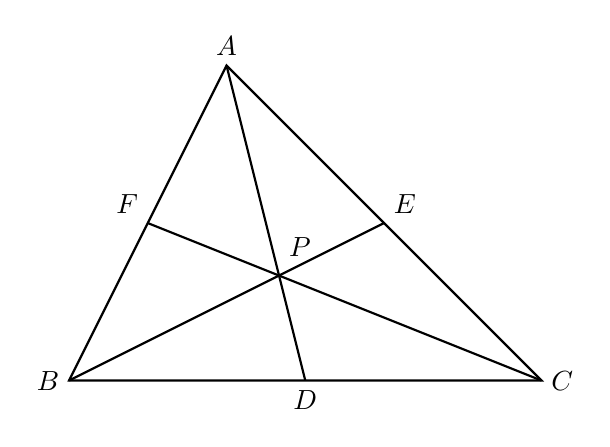
\begin{tikzpicture}
    \coordinate[label=left:$B$] (B) at (0,0) {};
    \coordinate[label=right:$C$] (C) at (6,0) {};
    \coordinate[label=above:$A$] (A) at (2,4) {};
    \draw [thick] (A) -- (B) -- (C) -- cycle;
    \coordinate[label=below:$D$] (D) at (3,0) {};
    \coordinate[label=30:$E$] (E) at (4,2) {};
    \coordinate[label=150:$F$] (F) at (1,2) {};
    \draw [thick] (A) -- (D);
    \draw [thick] (B) -- (E);
    \draw [thick] (C) -- (F);
    \node [label=80:$P$] at (2.65,1.33) {};
    \end{tikzpicture}
\end{figure}

\begin{thrm}{Menelaus' Theorem}{}
Given a triangle $\Delta ABC$, and a transversal that intersects $BC$, $AC$, $AB$ at points $D$, $E$, $F$ respectively. 
\begin{equation} \frac {AF}{FB} \times \frac {BD}{DC} \times \frac {CE}{EA} = 1 \end{equation} 
\end{thrm}

\begin{figure}[H]
    \centering
    \begin{tikzpicture}
    \coordinate[label=240:$C$] (C) at (0,0) {};
    \coordinate[label=below:$B$] (B) at (5,0) {};
    \coordinate[label=above:$A$] (A) at (2,4) {};
    \coordinate[label=-60:$D$] (D) at (9,0) {};
    \coordinate[label=135:$E$] (E) at (1,2) {};
    \draw (A) -- (B);
    \draw (C) -- (D);
    \draw (A) -- (C);
    \draw (D) -- (E);
    \node [label=80:$F$] at (4,1.33) {};
    \end{tikzpicture}
\end{figure}
\pagebreak

\section{Quadrilaterals}
\begin{thrm}{British Flag Theorem}{} 
If $ABCD$ is a rectangle and $P$ is a point inside of it, then we have 
\[ PA^2 + PC^2 = PB^2 + PD^2 \] 
\end{thrm}

\begin{figure}[H]
    \centering
    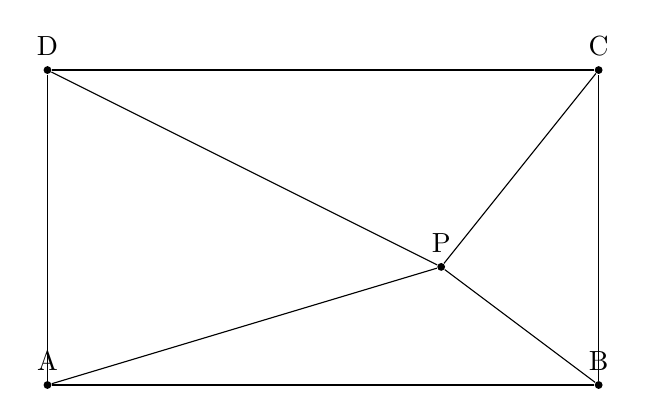
\begin{tikzpicture}[dot/.style={circle,inner sep=1pt,fill,label={#1},name=#1},
  extended line/.style={shorten >=-#1,shorten <=-#1},
  extended line/.default=1cm]
        \node [dot=A] at (0,0) {};
        \node [dot=B] at (7,0) {};
        \node [dot=C] at (7,4) {};
        \node [dot=D] at (0,4) {};
        \node [dot=P] at (5,1.5) {};
        \draw (A) -- (B) -- (C) -- (D) -- (A);
        \draw (P) -- (A);
        \draw (P) -- (B);
        \draw (P) -- (C);
        \draw (P) -- (D);
    \end{tikzpicture}
\end{figure}

\begin{proof}
This can be easily proven using Pythagoras' Theorem.
\end{proof}
\pagebreak

\section{Circle}
The reader should be familiar with basic circle terminology, such as \textbf{center}, \textbf{radius}, \textbf{chord}, \textbf{diameter}, \textbf{tangent}, \textbf{secant}, \textbf{arc}, \textbf{sector}, \textbf{segment}, and \textbf{circumference}.

\subsection{Angles}
Angle subtended at the centre of a circle by a chord is twice the angle subtended on the circumference.

All angles subtended by a fixed chord in the same segment of a circle are equal.

\subsection{Cyclic Quadrilaterals}
Angle chasing and cyclic quadrilaterals
\begin{thrm}{Ptolemy's Theorem}{}
Given a cyclic quadrilateral $ABCD$, the product of lengths of diagonals is equal to the sum of products of lengths of the pairs of the opposite sides: 
\begin{equation} AC \cdot BD = AB \cdot CD + AD \cdot BC \end{equation} 
\end{thrm}

\begin{figure}[H]
    \centering
    \includegraphics[width=6cm]{images/Ptolemys_theorem.jpg}
\end{figure}

\begin{thrm}{Ptolemy's Inequality}{}
For four points $A, B, C, D$ in the plane,
\begin{equation}
AB \cdot CD + BC \cdot DA \ge AC \cdot BD
\end{equation}
where equality holds if and only if $ABCD$ is a cyclic quadrilateral with diagonals $AC$ and $BD$, or if $A, B, C, D$ are collinear.
\end{thrm}

\begin{proof}
We construct a point $P$ such that the triangles $APB$ and $DCB$ are similar and have the same orientation. This means that
\begin{equation} \tag{1}
BD = \frac{BA \cdot DC}{AP}
\end{equation}

But since this is a spiral similarity, we also know that the triangles $ABD$ and $PBC$ are also similar, which implies that
\begin{equation} \tag{2}
BD = \frac{BC \cdot AD}{PC}
\end{equation}

By the triangle inequality, we have $AP + PC \ge AC$. Multiplying both sides of the inequality by $BD$ and using equations $(1)$ and $(2)$ gives us
\[ BA \cdot DC + BC \cdot AD \ge AC \cdot BD \]

which is the desired inequality. Equality holds iff $A$, $P$, $C$ are collinear. But since the triangles $BAP$ and $BDC$ are similar, this would imply that the angles $BAC$ and $BDC$ are congruent, i.e. that $ABCD$ is a cyclic quadrilateral.
\end{proof}

\begin{thrm}{Brahmagupta's Formula}{} 
Given a cyclic quadrilateral $ABCD$, \begin{equation} [ABCD] = \sqrt{(s-a)(s-b)(s-c)(s-d)} \end{equation} where $s$ denotes the semiperimeter. \end{thrm}
\pagebreak

\subsection{Power of a Point}
\textbf{Power of a point} is a frequently used tool in Olympiad geometry.

\begin{thrm}{Power of a point}{}
Let $\Gamma$ be a circle, and $P$ be a point. Let a line through $P$ meet $\Gamma$ at points $A$ and $B$, and another line through $P$ meet $\Gamma$ at points $C$ and $D$. Then 
\begin{equation}
PA \cdot PB = PC \cdot PD
\end{equation} 
\end{thrm}

\begin{figure}[H]
    \centering
    \includegraphics[width=12cm]{images/Power_of_a_point.png}
\end{figure}

\begin{proof}
There are two configurations to consider, depending on whether $P$ lies inside the circle or outside the circle.

When $P$ lies inside the circle, we have $\angle PAD = \angle PCB$ and $\angle APD = \angle CPB$, so triangles $PAD$ and $PCB$ are similar. Hence $\dfrac{PA}{PD} = \dfrac{PC}{PB}$. Rearranging, we get $PA \cdot PB = PC \cdot PD$.

When $P$ lies outside the circle, we have $\angle PAD = \angle PCB$ and $\angle APD = \angle CPB$, so again triangles $PAD$ and $PCB$ are similar. We get the same result in this case.
\end{proof}

As a special case, when $P$ lies outside the circle and $C=D$($PC$ is a tangent), we have \begin{equation} PA \cdot PB = PC^2 \end{equation}

\begin{figure}[H]
    \centering
    \includegraphics[width=6cm]{images/Power_of_a_point2.png}
\end{figure}
\pagebreak

\begin{thrm}{Converse to Power of a Point}{}
Let $A, B, C, D$ be four distinct points. Let lines $AB$ and $CD$ intersect at $P$. Assume that either (1) $P$ lies on both line segments $AB$ and $CD$, or (2) $P$ lies on neither line segments. Then $A, B, C, D$ are concyclic if and only if $PA \cdot PB = PC \cdot PD$.
\end{thrm}

\begin{proof}
The expression $PA \cdot PB = PC \cdot PD$ can be rearranged as $\dfrac{PA}{PD} = \dfrac{PC}{PB}$. In both configurations described in the statement of the theorem, we have $\angle APD = \angle CPB$. It follows by angles and ratios that triangles $APD$ and $CPB$ are similar.

Thus $\angle PAD = \angle PCB$. In both cases this implies that $A, B, C, D$ are concyclic.
\end{proof}

Suppose that $\Gamma$ has center $O$ and radius $r$. We say that the \textbf{power} of point $P$ with respect to $\Gamma$ is
\[ PO^2 - r^2 \]

Let line $PO$ meet $\Gamma$ at points $A$ and $B$, so that $AB$ is a diameter. We will use \emph{directed lengths}, meaning that for collinear points $P, A, B$, an expression such as $PA \cdot PB$ is assigned a positive value if $PA$ and $PB$ point in the same direction, and a negative value if they point in opposite directions. Then
\[ PA \cdot P B = (PO + OA)(PO + OB) = (PO-r)(PO+r) = PO^2 - r^2, \]
which is the power of $P$. So the power of a point theorem says that this quantity equals to $PC \cdot PD$, where $C$ and $D$ are the intersections with $\Gamma$ of any line through $P$.

By convention, the power of $P$ is negative when $P$ is inside the circle, and positive when $P$
is outside the circle. When $P$ is outside the circle, the power equals to the square of the length
of the tangent from $P$ to the circle.

\begin{figure}[H]
    \centering
    \includegraphics[width=8cm]{images/Power_of_a_point3.jpg}
\end{figure}

Let $\Gamma_1$ and $\Gamma_2$ be two circles with different centers $O_1$ and $O_2$, and radii $r_1$ and r$_2$ respectively.

The radical axis of $\Gamma_1$ and $\Gamma_2$ is the set of points with equal powers with respect to both circles.
\[ {PO_1}^2 - {r_1}^2 = {PO_2}^2 - {r_2}^2 \]
which can be represented as 
\[ pow(P, \Gamma_1) = pow(P, \Gamma_2). \]

The radical axis is a line perpendicular to the line connecting the circles' centers (line $\ell$).
\begin{proof}
\begin{lemma}
Let $P$ be a point in the plane, and let $P'$ be the foot of the perpendicular from $P$ to $O_1O_2$. Then \[ pow(P, \Gamma_1) - pow(P, \Gamma_2) = pow(P', \Gamma_1) - pow(P', \Gamma_2). \]
\end{lemma}
The proof of the lemma is an easy application of the Pythagorean Theorem.

\begin{lemma}
There is a unique point $P$ on line $O_1O_2$ such that $pow(P, O_1) = pow(P, O_2)$.
\end{lemma}

Proof: First show that $P$ lies between $O_1$ and $O_2$ via proof by contradiction, by using a bit of inequality theory and the fact that $O_1O_2 > r_1 + r_2$. Then, use the fact that $O_1P + PO_2 = O_1O_2$ (a constant) to prove the lemma.

The first lemma shows that every point on the plane can be equivalently mapped to a line on $O_1O_2$. The second lemma shows that only one point in this mapping satisfies the given condition. Combining these two lemmas shows that the radical axis is a line perpendicular to $\ell$, hence proved.
\end{proof}

When $\Gamma_1$ and $\Gamma_2$ intersect, the intersection points $A$ and $B$ both have a power of $0$ with respect to either circle, so $A$ and $B$ must lie on the radical axis. This shows that the radical axis \emph{coincides with the common chord} when the circles intersect.

To show that some point lies on the radical axis or the common chord, we can show that the point has \emph{equal powers with respect to the two circles}.

\begin{figure}[H]
    \centering
    \includegraphics[width=10cm]{images/Radical_axis.jpg}
    \caption{Radical axis}
\end{figure}

\begin{figure}[H]
    \centering
    \includegraphics[width=10cm]{images/Radical_center.jpg}
    \caption{Radical center}
\end{figure}

\begin{thrm}{Radical Axis Theorem}{}
Given three circles, no two concentric, the three pairwise radical axes (which are non-parallel) are concurrent, at a point known as the radical center.
\end{thrm}

\begin{proof}
Denote the three circles by $\Gamma_1, \Gamma_2, \Gamma_3$, and denote the radical axes of $\Gamma_i$ and $\Gamma_j$ by $\ell_{ij}$.

Suppose that the radical axes are not all parallel. Let $\ell_{12}$ and $\ell_{13}$ meet at $X$. Since $X$ lies on $\ell_{12}$, it has equal powers with respect to $\Gamma_1$ and $\Gamma_2$. Since X lies on $\ell_{13}$, it has equal powers with respect to $\Gamma_1$ and $\Gamma_3$. Therefore, $X$ has equal powers with respect to all three circles, and hence it must lie on $\ell_{23}$ as well.
\end{proof}

\subsection{Euler's Line and Nine-point Circle}
\begin{thrm}{Hamilton's theorem}{}
For $\triangle ABC$ with circumcenter $O$ and orthocenter $H$,
\[ \overrightarrow{OH} = \overrightarrow{OA} + \overrightarrow{OB} + \overrightarrow{OC} \]
\end{thrm}

\begin{thrm}{Euler line}{}
The circumcenter $O$, the centroid $G$ and the orthocenter $H$ are collinear.

In fact, we have 
\[ GH=2 OG \]
and
\[ OI^2 = R^2-2Rr \]
\end{thrm}

\begin{thrm}{Nine-point circle}{}
The midpoints of each side of the triangle, the feet of each altitude, and the midpoints of the line segments from each vertex to the orthocenter, all lie on a single circle.
\end{thrm}

The center of this circle lies on the Euler line, at the midpoint between the orthocenter and circumcenter.

The radius of this circle is half the circumradius of the triangle.

\subsection{Simson line}
\subsection{Miquel's theorem}
\begin{thrm}{Miquel's theorem}{}
Let $ABC$ be a triangle, and let $X, Y, Z$ be points on lines $BC, CA, AB$ respectively. Assume that the six points $A, B, C, X, Y, Z$ are all distinct. Then the circumcircles of triangles $AYZ, BZX, CXY$ pass through a common point.
\end{thrm}

\begin{proof}
The proof involves angle chasing.
\end{proof}

\pagebreak


\section*{Problems}
\begin{prbm}[Oxford MAT 2022]
100 circles all share the same centre, the $n$-th circle named as $C_n$. For each whole number $n$ between 1 and 99 inclusive, a tangent to circle $C_n$ intersects circle $C_{n+1}$ at two points, separated by a distance of 2.

Given that $C_1$ has radius 1, what is the radius of $C_{100}$?
\end{prbm}

\begin{proof}[Solution]
The relationship between circle $C_n$ of radius $r_n$ and circle $C_{n+1}$ of radius $r_{n+1}$ is shown below.
\begin{figure}[H]
    \centering
    \includegraphics[width=6cm]{images/c_n_circles.png}
\end{figure}

The tangent is at right angles to the radius, so there is a right-angled triangle with hypotenuse $r_n+1$ and other sides $r_n$ and $1$. Pythagoras gives ${r_{n+1}}^2 = {r_n}^2 + 1$. Since ${r_1}^2 = 1$, we have ${r_2}^2 = 2$ and ${r_3}^2 = 3$ and so on, up to ${r_{100}}^2 = 100$, so the radius of $C_100$ is 10.
\end{proof}
\pagebreak

\begin{prbm}
Prove that for angles $\alpha_1, \alpha_2, \dots, \alpha_n$ which satisfy the condition $0\degree \le a_i \le 180\degree$ for $i=1,2,\dots,n$ then
\[ \sin\alpha_1 + \sin\alpha_2 + \cdots + \sin\alpha_n \le n \sin\frac{\alpha_1+\cdots+\alpha_n}{n} \]
with equality iff $\alpha_1 = \cdots = \alpha_n$.
\end{prbm}

\begin{proof}
For 2 angles, 

\end{proof}

\chapter{Trigonometry}
\textbf{Readings:}
\begin{itemize}
\item \href{https://www.ams.org/books/prb/025/prb025-endmatter.pdf}{AMS}
\item \href{https://mathematicalolympiads.files.wordpress.com/2012/08/103-trigonometry-problems-titu-andreescu-zuming-feng.pdf}{Problems}
\end{itemize}

\section{Basic Definitions}
\textbf{Trigonometric functions} describe how the ratio of lengths vary according to the angle between the lengths.

For a triangle $\triangle ABC$ with $\angle C=90\degree$, we define \textbf{sine} as
\begin{equation}
\sin A=\frac{a}{c}
\end{equation}
and \textbf{cosine} as
\begin{equation}
\cos A=\frac{b}{c}.
\end{equation}
We define \textbf{tangent} as the ratio of sine and cosine; that is,
\begin{equation}
\tan A=\frac{\sin A}{\cos A}=\frac{a}{b}.
\end{equation}
We also define the reciprocals of the above trigonometric functions: \textbf{cosecant}, \textbf{secant} and \textbf{cotangent} are the reciprocals of sine, cosine and tangent respectively.
\begin{equation}
\cosec A=\frac{1}{\sin A}
\end{equation}
\begin{equation}
\sec A=\frac{1}{\cos A}
\end{equation}
\begin{equation}
\cot A=\frac{1}{\tan A}
\end{equation}

\section{Formulae}
\subsection{Pythagorean identities}
The following equation is known as the \textbf{Pythagorean identity}.
\begin{equation}\label{pythagorean_identity}
\sin^2 A + \cos^2 A = 1
\end{equation}
\begin{proof}
\[ \sin^2A+\cos^2A=\brac{\frac{a}{c}}^2+\brac{\frac{b}{c}}^2=\frac{a^2+b^2}{c^2} \]
By Pythagoras' Theorem, for a right-angled triangle, $a^2+b^2=c^2$. Hence we have our desired result.
\end{proof}
The following two equations are corollaries of \cref{pythagorean_identity}; they can be easily derived and shall be left as an exercise for the reader.
\[ \tan^2 A + 1 = \sec^2 A \]
\[ 1 + \cot^2 A = \cosec^2 A \]

\begin{exmp}{}{}
Compute $\sin^25\degree+\sin^210\degree+\cdots+\sin^290\degree$.
\end{exmp}
\begin{solution}
\begin{align*}
&\sin^25\degree+\sin^210\degree+\cdots+\sin^290\degree \\
&= (\sin^25\degree+\sin^285\degree) + \cdots + (\sin^240\degree+\sin^250\degree)+\sin^245\degree+\sin^290\degree \\
&= (\sin^25\degree+\cos^25\degree) + \cdots + (\sin^240\degree+\cos^240\degree)+\frac{1}{2}+1 \\
&= 8(1)+\frac{1}{2}+1 \\
&= \boxed{9\frac{1}{2}}
\end{align*}
\end{solution}

\subsection{Addition formulae}
\[ \sin (A \pm B) = \sin A \cos B \pm \cos A \sin B \]
\[ \cos (A \pm B) = \cos A \cos B \mp \sin A \sin B \]
\[ \tan (A \pm B) = \frac{\tan A \pm \tan B}{1 \mp \tan A \tan B} \]

\subsubsection{Double-angle formulae}
\[ \sin 2A = 2 \sin A \cos A \]
\[ \begin{split}
\cos 2A &= \cos^2 A - \sin^2 A \\
&= 2 \cos^2 A - 2 \\
&= 2 - 2 \sin^2 A
\end{split} \]
\[ \tan 2A = \frac{2 \tan A}{1 - \tan^2 A} \]

\subsubsection{Triple-angle formulae}
\[ \sin 3A = 3 \sin A - 4 \sin^3 A \]
\[ \cos 3A = 4 \cos^3 A- 3 \cos A \]
\[ \tan 3A = \frac{3\tan A-\tan^3A}{1-3\tan^2A} \]

\subsubsection{Half-angle formulae}
The following formulae are corollaries of \cref{pythagorean_identity}.
\[ \sin \frac{A}{2} = \pm \sqrt{\frac{1-\cos A}{2}} \]
\[ \cos \frac{A}{2} = \pm \sqrt{\frac{1+\cos A}{2}} \]

\subsubsection{Multiple-angle formulae}
Multiple-angle formulas are given by
\[ \sin nA = \sum_{k=0}^n \binom{n}{k} \cos^kA \sin^{n-k}A \sin\frac{n-k}{2}\pi \]
\[ \cos nA = \sum_{k=0}^n \binom{n}{k} \cos^kA \sin^{n-k}A \cos\frac{n-k}{2}\pi \]

\subsubsection{Sum to product}
\[ \sin A + \sin B = 2 \sin \frac{A+B}{2} \cos \frac{A-B}{2} \]
\[ \sin A - \sin B = 2 \cos \frac{A+B}{2} \sin \frac{A-B}{2} \]
\[ \cos A + \cos B = 2 \cos \frac{A+B}{2} \cos \frac{A-B}{2} \]
\[ \cos A - \cos B = -2 \sin \frac{A+B}{2} \sin \frac{A-B}{2} \]

\subsubsection{Product to sum}
\[ \sin A \cos B = \frac{1}{2}\sqbrac{\sin(A+B)+\sin(A-B)} \]
\[ \cos A \cos B = \frac{1}{2}\sqbrac{\cos(A+B)+\cos(A-B)} \]
\[ \sin A \sin B = -\frac{1}{2}\sqbrac{\cos(A+B)-\cos(A-B)} \]

\subsection{R-formula}
\[ a \sin \theta \pm b \cos \theta = \sin (\theta \pm \alpha) \]
\[ a \cos \theta \mp b \cos \theta = \cos (\theta \pm \alpha) \]
where $R = \sqrt{a^2 + b^2}$,
$\alpha = \tan^{-1} \dfrac{b}{a}$ where $0 < \alpha < \frac{\pi}{4}$.

\section{Theorems}
\begin{thrm}{Sine rule}{} 
\begin{equation}
\frac{a}{\sin A} = \frac{b}{\sin B} = \frac{c}{\sin C} = 2R
\end{equation} 
where $R$ denotes radius of circumcircle of triangle $ABC$. 
\end{thrm}

\begin{thrm}{Cosine rule}{} 
\begin{equation}
a^2 = b^2 + c^2 - 2bc \cos A
\end{equation} 
\end{thrm}

\begin{thrm}{Tangent law}{}
\begin{equation}
\frac{a-b}{a+b}=\frac{\tan\frac{A-B}{2}}{\tan\frac{A+B}{2}}
\end{equation}
\end{thrm}

\begin{thrm}{Cotangent law}{}
\begin{equation}
\cot A=\frac{b^2+c^2-a^2}{4S}
\end{equation}
\end{thrm}
\pagebreak

\section{Hyperbolic Functions}
\subsection{Basics}
The three main hyperbolic functions are:
\begin{equation}
\sinh x = \frac{e^x-e^{-x}}{2}
\end{equation}
\begin{equation}
\cosh x = \frac{e^x+e^{-x}}{2}
\end{equation}
\begin{equation}
\tanh x = \frac{e^x-e^{-x}}{e^x+e^{-x}} = \frac{e^{2x}-1}{e^{2x}+1}
\end{equation}

It is easy to see that
\[ \sinh x + \cosh x = e^x \]

\subsection{Reciprocals and Inverses}
Again these functions all have their inverse functions:
\begin{equation}
\sinh^{-1} x = \arsinh x = \ln(x+\sqrt{x^2+1})
\end{equation}
$\arsinh x$ has domain $x \ge 1$.

\begin{equation}
\cosh^{-1} x = \arcosh x = \ln(x+\sqrt{x^2-1})
\end{equation}
$\arcosh x$ has domain $x \ge 1$.

\begin{equation}
\tanh^{-1} x = \artanh x = \frac{1}{2}\ln(1+x)-\frac{1}{2}\ln(1-x)
\end{equation}
$\artanh x$ has domain $-1<x<1$.

As well as their reciprocal functions:
\begin{equation}
\cosech x = \frac{1}{\sinh x}
\end{equation}
\begin{equation}
\sech x = \frac{1}{\cosh x}
\end{equation}
\begin{equation}
\coth x = \frac{1}{\tanh x}
\end{equation}

\subsection{Identities}
Hyperbolic function identities have very similar forms to the trigonometric identities. 

However there is one key difference outlined in \textbf{Osborn's rule}: all the identities for the hyperbolic functions are exactly the same as the trigonometric identities, except whenever a product of two $\sinh$ functions is present we put a minus sign in front. For example if a trigonometric formula involved a $\sin^2x$, then the corresponding hyperbolic formula would contain a $-\sinh^2x$ instead.

\begin{table}[H]
\centering
\begin{tabular}{c|c}
\hline\hline
Trigonometric & Hyperbolic \\
\hline
$\cos^2\theta + \sin^2\theta = 1$ & $\cosh^2x - \sinh^2x = 1$ \\
$\sin(A \pm B) = \sin A \cos B \pm \cos A \sin B$ & $\sinh(A \pm B) = \sinh A \cosh B \pm \cosh A \sinh B$ \\
$\cos(A \pm B) = \cos A \cos B \mp \sin A \sin B$ & $\cosh(A \pm B) = \cosh A \cosh B \mp \sinh A \sinh B$ \\
$\cos 2\theta = \cos^2\theta - \sin^2\theta$ & $\cosh 2\theta = \cosh^2\theta + \sinh^2\theta$ \\
$\sin 2\theta = 2 \sin\theta \cos\theta$ & $\sinh 2\theta = 2 \sinh\theta \cosh\theta$ \\
$1 + \tan^2\theta = \sec^2\theta$ & $1 - \tanh^2\theta = \sech^2\theta$ \\
$1 + \cot^2\theta = \cosec^2\theta$ & $1 - \coth^2\theta = - \cosech^2\theta$ \\
\hline\hline
\end{tabular}
\end{table}
\pagebreak

\section*{Problems}
\begin{prbm}
Angles of $\triangle ABC$ satisfies
\[ \frac{\sin A+\sin B+\sin C}{\cos A+\cos B+\cos C}=\frac{12}{7} \]
and
\[ \sin A\sin B\sin C=\frac{12}{15}. \]
Given that $\sin C$ takes on three possible values $s_1,s_2,s_3$, find the value of $s_1s_2s_3$.
\end{prbm}
\begin{solution} \
\begin{align*}
\sin A+\sin B+\sin C
&= 2\sin\frac{A+B}{2}\cos\frac{A-B}{2}+\sin C \\
&= 2\sin\brac{90\degree-\frac{C}{2}}\cos\frac{A-B}{2}+2\sin\frac{C}{2}\cos\frac{C}{2} \\
&= 2\cos\frac{C}{2}\cos\frac{A-B}{2}+2\sin\frac{C}{2}\cos\frac{C}{2} \\
&= 2\cos\frac{C}{2}\brac{\cos\frac{A-B}{2}+\cos\frac{A+B}{2}} \\
&= 2\cos\frac{C}{2}\brac{2\cos\frac{A}{2}\cos\frac{B}{2}} 
= 4\cos\frac{A}{2}\cos\frac{B}{2}\cos\frac{C}{2}
\end{align*}
and
\begin{align*}
\cos A+\cos B+\cos C
&= 2\cos\frac{A+B}{2}\cos\frac{A-B}{2}+\cos C \\
&= 2\cos\brac{90\degree-\frac{C}{2}}\cos\frac{A-B}{2}+\cos2\brac{\frac{C}{2}} \\
&= 2\sin\frac{C}{2}\cos\frac{A-B}{2}+\brac{1-2\sin^2\frac{C}{2}} \\
&= 1+2\sin\frac{C}{2}\brac{\cos\frac{A-B}{2}-\sin\frac{C}{2}} \\
&= 1+2\sin\frac{C}{2}\brac{\cos\frac{A-B}{2}-\sin\brac{90\degree-\frac{A+B}{2}}} \\
&= 1+2\sin\frac{C}{2}\brac{\cos\frac{A-B}{2}-\cos\frac{A+B}{2}} \\
&= 1+2\sin\frac{C}{2}\brac{2\sin\frac{A}{2}\sin\frac{B}{2}} 
= 1+4\sin\frac{A}{2}\sin\frac{B}{2}\sin\frac{C}{2}
\end{align*}

This gives us the following simultaneous equations.
\[ \begin{cases}
\dfrac{\sin A+\sin B+\sin C}{\cos A+\cos B+\cos C} = \dfrac{4\cos\frac{A}{2}\cos\frac{B}{2}\cos\frac{C}{2}}{1+4\sin\frac{A}{2}\sin\frac{B}{2}\sin\frac{C}{2}} = \dfrac{12}{7} \\
\sin A\sin B\sin C = 8\brac{\sin\dfrac{A}{2}\sin\dfrac{B}{2}\sin\dfrac{C}{2}}\brac{\cos\dfrac{A}{2}\cos\dfrac{B}{2}\cos\dfrac{C}{2}} = \dfrac{12}{15}
\end{cases} \]

Solving, we get
\[ \begin{cases}
\sin\dfrac{A}{2}\sin\dfrac{B}{2}\sin\dfrac{C}{2}=\dfrac{1}{10} \\
\cos\dfrac{A}{2}\cos\dfrac{B}{2}\cos\dfrac{C}{2}=\dfrac{3}{5}
\end{cases} \]

We see that
\begin{align*}
\sin\frac{C}{2} &= \cos\frac{A+B}{2} = \cos\frac{A}{2}\cos\frac{B}{2} - \sin\frac{A}{2}\sin\frac{B}{2} \\
\sin^2\frac{C}{2}\cos\frac{C}{2} &= \frac{3}{5}\sin\frac{C}{2} - \frac{1}{10}\cos\frac{C}{2}
\end{align*}

Let $t=\cos\dfrac{C}{2}$. Then we get a quadratic equation. Solving it gives us 
\[ t=\sqrt{\frac{1}{2}}, \quad t=\sqrt{\frac{4}{5}}, \quad t=\sqrt{\frac{3}{10}}. \]

Hence $\boxed{s_1=1, s_2=\dfrac{4}{5}, s_3=\dfrac{3}{5}}$.
\end{solution}
\pagebreak

\begin{prbm}
Let 
\[ A = \cos^2 10\degree+\cos^2 50\degree - \sin40\degree\sin80\degree. \]
Determine the value of $A$.
\end{prbm}
\begin{solution}
Let $B=\sin^210\degree+\sin^250\degree-\cos40\degree\cos80\degree$.

Then
\begin{align*}
A+B &= 2-\cos40\degree \\
A-B &= (\cos^210\degree-\sin10\degree) + (\cos^250\degree-\sin^250\degree) + (\cos40\degree\cos80\degree-\sin40\degree\sin80\degree) \\
&= \cos20\degree + \cos100\degree + \cos(40\degree+80\degree) \\
&= \cos20\degree + \cos100\degree + \cos120\degree \\
&= 2\cos60\degree\cos40\degree - \cos60\degree \\
&= \cos40\degree - \frac{1}{2}
\end{align*}
Adding up the two equations gives us $2A=\dfrac{3}{2}$. Hence $\boxed{A=\dfrac{3}{4}}$.
\end{solution}
\pagebreak

\begin{prbm}[SMO Open]
Find the value of
\[ \frac{\tan40\degree\tan60\degree\tan80\degree}{\tan40\degree+\tan60\degree+\tan80\degree}. \]
\end{prbm}
\begin{solution}
We can show, more generally, that an acute $\triangle ABC$,
\[ \frac{\tan A\tan B\tan C}{\tan A+\tan B+\tan C}=1. \]
We see that
\begin{align*}
\tan A+\tan B+\tan 
&= \tan A+\tan B+\tan[180\degree-(A+B)] \\
&= \tan A+\tan B-\tan(A+B) \\
&= \tan A+\tan B-\frac{\tan A+\tan B}{1-\tan A\tan B} \\
&= (\tan A+\tan B)\brac{1-\frac{1}{1-\tan A\tan B}} \\
&= (\tan A+\tan B)\brac{-\frac{\tan A\tan B}{1-\tan A\tan B}} \\
&= \tan A\tan B\brac{-\frac{\tan A+\tan B}{1-\tan A\tan B}} \\
&= \tan A\tan B[-\tan(A+B)] \\
&= \tan A\tan B\tan[180\degree-(A+B)] \\
&= \tan A\tan B\tan C
\end{align*}
Hence proven.
\end{solution}
\pagebreak

\begin{prbm}[Oxford MAT]
Evaluate 
\[ \sin^2 1\degree + \sin^2 2\degree + \dots + \sin^2 89\degree + \sin^2 90\degree. \]
\end{prbm}

\begin{proof}[Solution]
Recall the Pythagorean Identity $\sin^2 x + \cos^2 x = 1$.

Rewriting and pairing up terms gives us 
\begin{align*}
&\sin^2 1\degree + \sin^2 2\degree + \dots + \cos^2 2\degree + \cos^2 1\degree + 1 \\
&= (\sin^2 1\degree + \cos^2 1\degree) + \dots + (\sin^2 44\degree + \cos^2 44\degree) + \sin^2 45\degree + 1 \\
&= 44(1) + \frac{1}{2} + 1 = \boxed{45\frac{1}{2}}
\end{align*}
\end{proof}

\chapter{Coordinate Systems}
\section{Cartesian Coordinates}
\subsection{Basics}
The coordinate plane is determined by two \textbf{axes} -- a horizontal $x$-axis and a vertical $y$-axis; both axes intersect at a point called the \textbf{origin}. Each point in the coordinate plane can be specified by an ordered pair of numbers $(x,y)$.

The \textbf{gradient} of a line with points $(x_1, y_1)$ and $(x_2, y_2)$ is given by
\begin{equation}
m = \frac{y_2-y_1}{x_2-x_1}
\end{equation}

Given gradient $m$ and $y$-intercept $c$, a line can be represented in the point-slope form:
\begin{equation}
y=mx+c
\end{equation}

Given gradient $m$ and a point on the line $(x_1,y_1)$, a line can be represented as
\begin{equation}
y-y_1=m(x-x_1)
\end{equation}

For two \textbf{parallel} lines, they have the same gradients.

For two \textbf{perpendicular} lines, the product of the gradients is $-1$.

The distance from a point $(m, n)$ to the line $Ax + By + C = 0$ is given by
\[ d = \frac{Am+Bn+C}{\sqrt{A^2+B^2}} \]

The distance between two lines is given by


The area of polygon is given by


reflection of point, line about line

\subsection{Conic Sections}
Definitions and basic properties of conic sections - refer to F maths
\subsubsection{Standard Equations of Conics}
Conic sections are the family of curves obtained by intersecting a cone with a plane. This intersection can take different forms according to the angle the intersecting plane makes with the side of the cone. The standard conic sections are the circle, the parabola, the ellipse and the hyperbola. There are also special cases, such as a point or a line, however these are trivial (sometimes called degenerate) so we shall not cover them.

\begin{table}[H]
\centering
\renewcommand{\arraystretch}{1.8}
\begin{tabular}{c|c|c}
\hline\hline
Conic & Cartesian equation & Parametric equation \\
\hline
Circle & $x^2+y^2=a^2$ & $x=\cos t, y=\sin t$ \\
Parabola & $x=4ay^2$ & $x=4at^2, y=t$ \\
Ellipse & $\frac{x^2}{a^2}+\frac{y^2}{b^2}=1$ & $x=a\cos t, y=b\sin t$ \\
Hyperbola & $\frac{x^2}{a^2}-\frac{y^2}{b^2}=1$ & $x=b\tan t, y=a\sec t$ \\
\hline\hline
\end{tabular}
\end{table}

\begin{remark}
The circle is a special case of the ellipse, where $a=b$.
\end{remark}

\subsubsection{Recognising Conics}
The general equation of any conic is $Ax^2 + Bxy + Cy^2 + Dx + Ey + F = 0$. When we see an equation like this we know that it describes a conic, but to find out which conic it describes one has to manipulate the equation into one of the equations given above.

One method is to sketch a phase plot which is a graph drawn up from the given equation to allow us to try understand what the equation describes in a physical system. In many cases we can manipulate the given equation to take the form of a conic.
\pagebreak

\section{Polar Coordinates}
You will already be familiar with coordinates in the form $(x, y)$ meaning that we move $x$ units in the $x$-direction (along the $x$-axis) and $y$ in the $y$-direction (along the $y$-axis). These are Cartesian coordinates on the $xy$-plane. Although Cartesian coordinates are very useful, there are sometimes situations where it is much easier to use another coordinate system called \textbf{polar coordinates}. These are coordinates in the form $(r,\theta)$ where $r$ is the distance to the point from the origin and $\theta$ is the angle in radians between the positive $x$-axis and the line formed by $r$.

From trigonometry and Pythagoras' theorem there are the following relationships:
\[ x = r\cos\theta \quad y = r\sin\theta \quad r = \sqrt{x^2+y^2} \]
We can use the formulae above to allow us to convert between Polar and Cartesian coordinates.

\section{Barycentric Coordinates}
\subsection{Basics}
\subsubsection{The Coordinates}
\begin{defn}{}{}
Each point in the plane is assigned an ordered triple of real numbers $P = (x, y, z)$ such that
\[ \vec{P} = x\vec{A} + y\vec{B} + z\vec{C} \quad \text{and} \quad x + y + z = 1 \]
\end{defn}
% https://web.evanchen.cc/handouts/bary/bary-full.pdf

\subsubsection{Lines}
\pagebreak

\section{Complex Numbers}

\chapter{Advanced Techniques}
\section{Inversion in the plane}
Definition and first properties
Generalised lines and circles
Inversion distance formula
O Inversive geometry

\section{Projective geometry}
Cross ratios
Projective transformations
O Projective geometry, e.g. cross ratios, harmonic bundles, poles and polars,
Pascal's theorem, and so on

\subsection{Homothety}

\section{Complete quadrilaterals}
Spiral similarity
Miquel point of a cyclic quadrilateral


\part{Combinatorics}
basics of counting; the inclusion-exclusion principle; the pigeonhole principle; permutations and combinations; the binomial theorem; recurrence relations and linear recurrence relations; 

\chapter{Combinatorics}
\begin{itemize}
\item \href{https://rainymathboy.files.wordpress.com/2011/01/102-combinatorial-problems.pdf}{102 Combinatorial Problems From The Training of The USA IMO Team}
\end{itemize}

" Recursion and recurrence relations
" Definition of sets and functions
O Elementary probability
O Expected value and linearity of expectation
O Basic properties and definitions from graph theory, e.g. connectedness and degree of a vertex
O Definition and existence of the convex hull of a finite set of points % https://ti.inf.ethz.ch/ew/courses/CG13/lecture/Chapter%203.pdf
!! Nontrivial results from graph theory, such as Hall's marriage lemma or Turan’s theorem
\pagebreak

\section{Permutations and Combinations}
A \textbf{permutation} is an arrangement of objects in a specific order. Number of ways to permute $k$ of $n$ items:
\[ \per{n}{k} = \frac{n!}{(n-k)!} \]

A \textbf{combination} is a selection of objects without regard to the order. Number of ways to choose $k$ ok $n$ items:
\[ \com{n}{k} = \binom{n}{k} = \frac{n!}{k!(n-k)!} \]

Number of subsets of a set with $n$ elements is $2^n$.

Number of ways to choose $k$ objects from $n$ objects if repetition is allowed = $\binom{n+k-1}{k}$.

Number of paths from $(0,0)$ to $(m,n)$ going 1 unit rightwards or upwards = $\binom{m+n}{n}$.

Number of $k$-tuples of positive integers which sum equals $n$ is $\binom{n-1}{k-1}$.

Number of $k$-tuples of non-negative integers which sum equals $n$ is $\binom{n+k-1}{k-1}$.

\subsection{Stars and Bars}
The setup is the following: suppose there are three children $c_1$, $c_2$, $c_3$, and we distribute 10 identical candies among these three children. Each child can receive any number of candies, including 0. For example, one possible distribution is $(4,3,3)$: in this case, $c_1$ receives 4 candies, $c_2$ receives 3, and $c_3$ receives 3. How many ways can we distribute the candies?

The key observation is the following: we can distribute the candies by arranging them in a line, and then placing two ``bars" somewhere along the line. For example, the $(4,3,3)$ described above can be modeled by the following:
\[ \ast\ast\ast\ast | \ast\ast\ast | \ast\ast\ast \]
Each $\ast$ represents a candy, and the two location of the two bars determines the distribution of the candies. Notice that the following distribution is also possible:
\[ ||\ast\ast\ast\ast\ast\ast\ast\ast\ast\ast \]
The above diagram corresponds to the distribution $(0,0,10)$. In general, $c_1$ receives the candies left of the first bar, $c_2$ receives the candies between the two bars, and $c_3$ receives the candies right of the second bar.

So we can see that distributing candies is identical to choosing the location of the two bars to place in $10+2=12$ empty slots, hence $\binom{12}{2}$ ways.

In general, if there are $n$ candies and $k$ children, then there are $n+k-1$ slots, and we must place $k-1$ bars. The remaining $n$ candies, interspersed among the bars, represent a istribution.
Thus, the number of distributions is
\[\binom{n+k-1}{k-1}.\]
\pagebreak

\section{Combinatorial Identities}
\subsection{Pascal's Triangle}
We can observe that by means of expansion,
\begin{equation} \binom{n}{k} = \binom{n}{n-k} \end{equation}

Each number in the Pascal's triangle is a binomial coefficient. Pascal's and hockey-stick identities:
\begin{equation} 
\binom{n}{k} + \binom{n}{k+1} = \binom{n+1}{k+1} 
\end{equation}
\begin{equation}
\sum_{r=k}^{n} \binom{r}{k} = \binom{n+1}{k+1}
\end{equation}
\begin{equation}
\sum_{r=0}^{n} \binom{k+r}{r} = \binom{n+k+1}{n}
\end{equation}

We also have 
\begin{equation}
\binom{n}{k} \binom{k}{m} = \binom{n}{m} \binom{n-m}{k-m}
\end{equation}
which can be easily proven via expansion.

\begin{thrm}{Vandermonde's Identity}{}
\begin{equation}
\sum_{r=0}^{k} \binom{m}{r} \binom{n}{k-r} = \binom{m+n}{k}
\end{equation}
\end{thrm}

\subsection{Binomial Theorem}
\begin{thrm}{Binomial Theorem}{} 
For $n \in \ZZ^{+}$ and $a,b\in\RR$, 
\begin{equation}
\begin{split}
(a+b)^n &= \sum_{k=0}^n\binom{n}{k}a^{n-k}b^k\\
&= \binom{n}{0}a^n + \binom{n}{1}a^{n-1}b + \cdots + \binom{n}{n}b^n
\end{split}
\end{equation}
\end{thrm}

\begin{proof}
This can be proven using mathematical induction.
\end{proof}

\begin{corollary}
For all $n\in\ZZ^{+}$, the following equality holds:
\begin{equation}
2^n = \sum_{k=0}^{n} \binom{n}{k} = \binom{n}{0}+\binom{n}{1}+\cdots+\binom{n}{n}
\end{equation}
\end{corollary}
\begin{remark}
The above identity simply follows by $a = b = 1$.
\end{remark}
We give an alternate proof below that relates this identity to the set of subsets of a set.
\begin{proof}
Let $A$ be a set with $n$ elements, and let $A_k$ denote the subset of the power set $2_A$ containing the subsets of $A$ of size $k$. Then the sets $A_0,A_1,\dots,A_n$ partition $2^A$, which means the following
equalities hold:
\begin{align*}
2^n=|2^A| &= |A_0|+|A_1|+\cdots+|A_n| \\
&= \binom{n}{0}+\binom{n}{1}+\cdots+\binom{n}{n} = \sum_{k=0}^{n} \binom{n}{k}
\end{align*}
In other words, every subset of $A$ has a size in $\{0,1,\dots,n\}$, so to count the number of subsets of $A$, we can count the number of subsets of each size over all possible sizes.
\end{proof}

Sums:
\begin{equation}
\sum_{k=0}^{n} k \binom{n}{k} = n 2^{n-1}
\end{equation}
\begin{equation}
\sum_{k=0}^{n} k^2 \binom{n}{k} = n(n+1) 2^{n-2}
\end{equation}
\pagebreak

\section{Cardinality Rules and Principles}
In this section, we will see the formalization of counting strategies that we often take for granted: the product rule, the sum rule, and the pigeonhole principle.

\subsection{Product Rule}
% https://courses.cs.duke.edu/spring19/compsci230/Notes/lecture22.pdf

\subsubsection{Examples of counting}
Counting number of rectangles:

For a $m \times n$ grid, to form a rectangle, choose $2$ points from the $m+1$ points along the column, and choose $2$ points from the $n+1$ points along the row. Hence the number of rectangles we can form is \[ {m+1 \choose 2}{n+1 \choose 2} \]

Circle division: chords divide a circle
number of chords = n choose 2 where there are n points
number of intersection points = n choose 4 (any 4 points forms 2 chords, thus gives a unique intersection point)

\subsection{Principle of Inclusion-Exclusion}
The \textbf{principle of inclusion and exclusion} is a counting technique that computes the number of elements that satisfy at least one of several properties while guaranteeing that elements satisfying more than one property are not counted twice.

The idea behind this principle is that summing the number of elements that satisfy at least one of two categories and subtracting the overlap prevents double counting.

For two sets, 
\[ |A \cup B| = |A| + |B| - |A \cap B| \] 
where $|S|$ denotes the cardinality (i.e. number of elements) of set $S$.

For three sets,  \[ |A \cup B \cup C| = |A| + |B| + |C| - |A \cap B| - |B \cap C| - |C \cap A| + |A \cap B \cap C| \]

More generally, if $A_i$ are finite sets, then
\begin{equation} 
\begin{aligned} |\bigcup_{i=1}^{n} A_i| = &\sum_{i=1}^{n} |A_i| - \sum_{1 \le i \le j \le n} |A_i \cap A_j| + \sum_{1 \le i \le j \le k \le n} |A_i \cap A_j \cap A_k|\\
&- \cdots + (-1)^{n-1} |A_1 \cap \cdots \cap A_n|. 
\end{aligned} 
\end{equation}

\begin{exmp}{}{}
Find the number of integers from the set $\{1,2,\dots,1000\}$ which are divisible by 3 or 5.
\end{exmp}

\begin{proof}[Solution]
Let
\begin{align*}
S &= \{1,2,\dots,1000\} \\
A &= \{x\in S\:|\:x\text{ is divisible by 3}\} \\
B &= \{x\in S\:|\:x\text{ is divisible by 5}\}
\end{align*}
It follows that \[ A\cap B = \{x\in S\:|\:x\text{ is divisible by 15}\} \]
Observe that
\begin{quote}
for any two natural numbers $n$ and $k$ with $n\ge k$, the number of integers in the set $\{1,2,\dots,n\}$ which are divisible by $k$ is $\floor{\dfrac{n}{k}}$
\end{quote}
Hence we have 
\begin{align*}
|A\cup B| &= |A| + |B| - |A\cap B| \\
&= \floor{\frac{1000}{3}} + \floor{\frac{1000}{5}} - \floor{\frac{1000}{15}} \\
&= 333 + 200 - 66 = \boxed{467}
\end{align*}
\end{proof}

\subsection{Pigeonhole Principle}
\begin{thrm}{Pigeonhole Principle}{}
If $k+1$ objects are placed into $k$ boxes, then at least one box contains two or more objects. 
\end{thrm}

\begin{proof}
We use a proof by contraposition.

Suppose none of the $k$ boxes has more than one object. Then the total number of objects would be at most $k$. This contradicts the statement that we have $k + 1$ objects.
\end{proof}

\begin{thrm}{Generalised Pigeonhole Principle}{} 
If $n$ objects are placed into $k$ boxes, then there is at least one box containing at least $\ceiling{\frac{n}{k}}$ objects. 
\end{thrm}

\begin{proof}
We use a proof by contradiction.

Suppose that none of the boxes contains more than $\ceiling{\dfrac{n}{k}} - 1$ objects.

Then the total number of objects is \[k\brac{\ceiling{\frac{n}{k}}-1}\] but \[ k\brac{\ceiling{\frac{n}{k}} - 1} < k \sqbrac{\brac{\frac{n}{k} + 1} - 1} = n \]
where the inequality $\ceiling{\dfrac{n}{k}} < \dfrac{n}{k}+1$ was used.

This is a contradiction, because there are a total of $n$ objects.
\end{proof}
\pagebreak

\section{Catalan Numbers}
%https://brilliant.org/wiki/catalan-numbers/
\begin{thrm}{Catalan numbers}{}
The Catalan numbers are given by the formula
\begin{equation}
C_n = \frac{1}{n+1} \binom{2n}{n}
\end{equation}
\end{thrm}

\subsection{Dyck Paths and Acceptable Sequences}
The number of valid parenthesis expressions that consist of n right parentheses and n left parentheses is equal to the $n$-th Catalan number. 

For example, $C_3 = 5$ and there are 5 ways to create valid expressions with 3 sets of parenthesis:
\begin{itemize}
    \item ( ) ( ) ( )
    \item ( ( ) ) ( )
    \item ( ) ( ( ) )
    \item ( ( ( ) ) )
    \item ( ( ) ( ) )
\end{itemize}

Considering right parenthesis to be $+1$s, and left $-1$s, we can write this more formally as follows:

The number of sequences $a_1, \dots, a_n$ of $2n$ terms that can be formed using $n$ copies of $+1$s and $n$ copies of $-1$s whose partial sums satisfy

\subsection{Recurrence Relation; Generating Function}

\pagebreak

\section{Derangements}
A derangement is a permutation with no fixed points. That is, a derangement of a set leaves no element in its original place. For example, the derangements of $\{1,2,3\}$ are $\{2, 3, 1\}$ and $\{3, 1, 2\}$, but $\{3,2, 1\}$ is not a derangement of $\{1,2,3\}$ because $2$ is a fixed point.\\
The number of derangements of an $n$-element set is denoted $D_n$. This number satisfies the recurrences \[D_n = n \cdot D_{n - 1} + (-1)^n\]
and \[D_n = (n - 1)\cdot (D_{n - 1} + D_{n - 2})\]
and is given by the formula \[D_n = n! \sum_{k=0}^{n} \frac{(-1)^k}{k!}.\]
\pagebreak

\section{Probability}
\pagebreak

\section*{Problems}
\begin{prbm}[Langford's Problem $L(n)$]
Given the multiset\footnote{A multiset is like a set except that there may be more than one occurrence of an element.} of positive integers:
\[ \{1,1,2,2,3,3,\dots,n,n\},\]
can they be arranged in a sequence such that for $1 \le i \le n$ there are $i$ numbers between the two occurrences of $i$?
\end{prbm}

\begin{proof}

% https://link.springer.com/content/pdf/10.1007/978-3-031-13566-8_9.pdf
% https://www.youtube.com/watch?v=Lju6aYms2EA

\end{proof}
\pagebreak

\begin{prbm} 
Use a combinatorial proof to show that 
\[ \sum_{k=0}^{n} \binom{n}{k}\binom{n}{n-k} = \binom{2n}{n}. \] 
\end{prbm}

\begin{proof}
For combinatorial proofs, we begin with a story. Consider a group of $2n$ animals, where $n$ are dogs and $n$ are cats.

\textbf{RHS:} Number of ways to pick $n$ animals from a group of $2n$ animals.

For LHS, we try to understand what's going on in the summation:
\[ \sum_{k=0}^{n} \binom{n}{k}\binom{n}{n-k} = \binom{n}{0}\binom{n}{n} + \binom{n}{1}\binom{n}{n-1} + \cdots \]

We see that each term looks like a case. For example, for the first term, pick $0$ items from the first group, and pick $n$ items from the second group. This shows that if we want to pick $n$ animals, we can pick $k$ dogs and $n-k$ cats.

\textbf{LHS:} Consider all cases where we pick $k$ dogs and $n-k$ cats.

$\therefore$ LHS is the same as RHS as they both count the same number of things. Hence proven.
\end{proof}
\pagebreak

\begin{prbm} 
Evaluate 
\[ S = {n \choose 1} + 2 {n \choose 2} + 3 {n \choose 3} + \cdots + n {n \choose n}. \] 
\end{prbm}

\begin{proof}[Solution]
Writing the sum backwards yields 
\begin{align*} 
S &= n {n \choose n} + (n-1) {n \choose n-1} + \cdots + {n \choose 1} \\&= n {n \choose 0} + (n-1) {n \choose 1} + \cdots + {n \choose n-1} 
\end{align*} 
Add this to the original series gives us 
\begin{align*}
2S &= n \left[{n \choose 0} + {n \choose 1} + \cdots + {n \choose n}\right]\\ 
2S &= n 2^n \\
\Aboxed{S &= n 2^{n-1}}
\end{align*}
\end{proof}
This is the proof of the sum
\[ \sum_{k=0}^{n} k \binom{n}{k} = n 2^{n-1} \]
\pagebreak

\begin{prbm}[USAMO 2005]
Legs $L_1, L_2, L_3, L_4$ of a square table each have length $n$, where $n$ is a positive integer. For how many ordered 4-tuples $(k_1, k_2, k_3, k_4)$ of non-negative integers can we cut a piece of length $k_i$ from the end of leg $L_i \; (i=1,2,3,4)$ and still have a stable table?

(The table is stable if it can be placed so that all four of the leg ends touch the floor. Note that a cut leg of length $0$ is permitted.)
\end{prbm}

\begin{proof}[Solution]
The table is stable if $k_1+k_3=k_2+k_4$. Let this common value be $k$ such that that $k_1+k_3=k_2+k_4=k$. Let $c_k$ be the number of ways to make the table stable for each value of $k$. We want to find $\sum_{k=0}^{2n}c_k$.

Note that each table leg is at least 0 and at most $n$, hence we'll break this into two sums so that it's easier to handle:
\[\sum_{k=0}^n c_k+\sum_{k=n+1}^{2n}c_k\]

\textbf{Case 1}: If $0\le k\le n$, there are $k+1$ ways to partition $k_1$ and $k_3$, and another $k+1$ ways to partition $k_2$ and $k_4$. There are $(k+1)^2$ ways to partition $k_i$ in this interval. Hence 
\[\sum_{k=0}^n (k+1)^2\]

\textbf{Case 2}: If $n+1\le k\le 2n$, each of the $k_i$ is at most $n$ and at least $0$. There are $(2n-k+1)^2$ ways to partition the $k_i$ in this interval. Hence
\[\sum_{k=n+1}^{2n}(2n-k+1)^2\]

Evaluating the sum gives us $\boxed{\frac{(n+1)(2n^2+4n+3)}{3}}$.
\end{proof}

\part{Miscellaneous}
\chapter{Proofs}
\section{Induction}
\begin{defn}{Mathematical induction}{}
Let $P(n)$ be a family of statements indexed by $n \in \NN$.

By \vocab{mathematical induction}, If $P(0)$ is true and $P(k)$ is true $\forall k \in \NN$, then $P(n)$ is true $\forall n \in \NN$.\end{defn}

Steps to write the proof:
\begin{enumerate}
  \item \textbf{Base case.}
  
  Prove that $P(0)$ is true.
  \item \textbf{Inductive step.}.
  
  $P(k) \implies P(k+1)$
\end{enumerate}

\begin{exmp} Prove that \[ 1 + 2 + 3 + \cdots + n = \frac{n(n+1)}{2} \] for all positive integers $n$. \end{exmp}
\begin{proof} \ {\\}
The statement is true for $n=1$ (base case) because with $n=1$, LHS = RHS = $1$.

Assume that the statement is true for some $n=k$, where $k \in \ZZ^{+}$. By our induction hypothesis, we have $1 + 2 + 3 + \cdots + k = \dfrac{k(k+1)}{2}$.

To show that the statement is true for $k+1$, 
\begin{align*}
1 + 2 + 3 + \cdots + k + (k+1) &= \frac{k(k+1)}{2} + (k+1)\\
&= \frac{(k+1)(k+2)}{2}\\
&= \frac{(k+1)[(k+1)+1]}{2}
\end{align*}
$\because$ The statement holds true for $n=k$ and $n=k+1$, 

$\therefore$ The statement is true for all positive integers $n$. 
\end{proof}

\begin{defn}{Cauchy induction}{}
\vocab{Cauchy induction}, also known as forward-backward induction, is a variant of mathematical induction.
\end{defn}

To write the proof, there are a few steps:
\begin{enumerate}
  \item \textbf{Base case.}
  
  Prove that $P(0)$ is true.
  \item \textbf{Inductive step}.
  
  $P(k) \implies P(2k)$
  
  $P(k) \implies P(k-1)$
\end{enumerate}

\chapter{Calculus}
\section{Riemann Sums}
Given $y=f(x)$, we want to find the integral on the $x$-interval $[0,1]$.

Split the interval $[0,1]$ into $n$ equal subintervals \[ \left[0, \frac{1}{n}\right], \left[\frac{1}{n}, \frac{2}{n}\right], \cdots, \left[\frac{n-1}{n}, 1\right]. \]

\begin{figure}[H]
    \centering
    \includegraphics[width=6cm]{images/Riemanns_sums.png}
\end{figure}

Consider the height of the rectangles. We take the right value. Hence for the $k$-th subinterval $\sqbrac{\dfrac{k-1}{n}, \dfrac{k}{n}}$ where $k=1,\dots,n$, the height of rectangle is $f\left(\dfrac{k}{n}\right)$.\\

Area of $k$th rectangle is 
\[ \frac{1}{n} \cdot f\left(\frac{k}{n}\right).\]

Therefore, the integral is obtained by summing up the area of $n$ rectangles, which gives us
\begin{equation} 
\int_{0}^{1} f(x) \dd{x} = \lim_{n \to \infty} \sum_{k=1}^{n} \frac{1}{n} f\brac{\frac{k}{n}} 
\end{equation}
where there are infinitely many rectangles, i.e. $n \to \infty$.
\pagebreak

\section*{Problems}
\begin{prbm}[SMO 2020 Open Q10]
Find the value of 
\[ S = \lim_{n \to \infty} \sum_{k=1}^{n} \frac{1}{\sqrt{n(n+k)}} \]
\end{prbm}
    
\begin{solution}
\begin{align*}
S &= \lim_{n \to \infty} \sum_{k=1}^{n} \frac{1}{n} \sqrt{\frac{1}{1+\frac{k}{n}}}\\
&= \int_{0}^{1} \frac{1}{\sqrt{1+x}} \dd{x}\\
&= 2\sqrt{2} - 2
\end{align*}
\end{solution}

\begin{prbm}[SMO 2018 Open Q12]
Given that
\[ S=\lim_{n\to\infty}\sum_{k=1}^n\frac{1}{n+k} \]
Find the value of $S$.
\end{prbm}
\begin{solution}
Using Riemann sums,
\[ \lim_{n\to\infty}\sum_{k=1}^nf\brac{\frac{k}{n}} = \int_0^1f(x)\dd{x} \]
Hence
\[ S = \lim_{n\to\infty}\frac{1}{n}\sum_{k=1}^n\frac{1}{1+\frac{k}{n}} = \int_0^1\frac{1}{1+x}\dd{x} = \boxed{\ln2} \]
\end{solution}


\end{document}